%%%% Time-stamp: <2018-03-24 14:05:09 vk>
%% ========================================================================
%%%% Disclaimer
%% ========================================================================
%%
%% created by
%%
%%      Karl Voit
%%

%% ========================================================================
%%%% Basic settings
%% ========================================================================
%% (idea of using newcommands for basic documentclass settings from: Thomas Schlager)

\newcommand{\mypapersize}{A4}
%% e.g., "A4", "letter", "legal", "executive", ...
%% The size of the paper of the resulting PDF file.

\newcommand{\mylaterality}{twoside}
%% "oneside" or "twoside"
%% Either you are creating a document which is printed on both, left pages
%% and right pages (twoside) or you create a document which is printed
%% on right pages only (oneside).

\newcommand{\mydraft}{false}
%% "true" or "false"
%% Use draft mode? If true, included graphics are replaced by empty
%% rectangles (of same size) and overfull boxes (in margin space) are
%% marked with black box (-> easy to spot!)

\newcommand{\myparskip}{half}
%% e.g., "no", "full", "half", ...
%% How to separate paragraphs: indention ("no") or spacing ("half",
%% "full", ...).

\newcommand{\myBCOR}{0mm}
%% Inner binding correction. This value depends on the method which is
%% being used to bind your printed result. Some techniques do not
%% require a binding correction at all ("0mm"), other require for
%% example "5mm". Refer to KOMA script documentation for a detailed
%% explanation what a binding correction is and how to measure it.

\newcommand{\myfontsize}{12pt}
%% e.g., 10pt, 11pt, 12pt
%% The font size of the main text in pt (points).

\newcommand{\mylinespread}{1.0}
%% e.g., 1.0, 1.5, 2.0
%% Line spacing in %/100. For example 1.5 means 150% of the usual line
%% spacing. Please use with caution: 100% ("1.0") is fine because the
%% font was designed for it.

\newcommand{\mylanguage}{ngerman,american}
%% "english,ngerman", "ngerman,english", ...
%% NOTE: The *last* language is the active one!
%% See babel documentation for further details.

%% BibLaTeX-settings: (see biblatex reference for further description)
\newcommand{\mybiblatexstyle}{authoryear}
%% e.g., "alphabetic", "authoryear", ...
%% The biblatex style which is being used for referencing. See
%% biblatex documentation for further details and more values.
%%
%% CAUTION: if you change the style, please check for (in)compatible
%%          "biblatex" package options in the file
%%          "template/preamble.tex"! For example: "alphabetic" does
%%          not have an option "dashed=..." and causes an error if it
%%          does not get removed from the list of options.

\newcommand{\mybiblatexdashed}{false}  %% "true" or "false"
%% If true: replace recurring reference authors with a dash.

\newcommand{\mybiblatexbackref}{true}  %% "true" or "false"
%% If true: create backward links from reference to citations.

\newcommand{\mybiblatexfile}{references-biblatex.bib}
%% Name of the biblatex file that holds the references.

\newcommand{\mydispositioncolor}{30,103,182}
%% e.g., "30,103,182" (blue/turquois), "0,0,0" (black), ...
%% Color of the headings and so forth in RGB (red,green,blue) values.
%% NOTE: if you are using "0,0,0" for black, printers might still
%%       recognize pages as color pages. In case this is a problem
%%       (paying for color print-outs vs. paying for b/w-printouts)
%%       please edit file "template/preamble.tex" and change
%%       "\definecolor{DispositionColor}{RGB}{\mydispositioncolor}"
%%       to "\definecolor{DispositionColor}{gray}{0}" and thus
%%       overwriting the value of \mydispositioncolor above.

\newcommand{\mycolorlinks}{true}  %% "true" or "false"
%% Enables or disables colored links (hyperref package).

\newcommand{\mytitlepage}{template/title_Thesis_TU_Graz}
%% Your own or one of following pre-defined title pages:
%% "template/title_plain_maketitle": simple maketitle page
%% "template/title_Diplomarbeit_KF_Uni_Graz.tex": fancy (german) title page for KF Uni Graz
%% "template/title_Thesis_TU_Graz":
%%             titlepage for Graz University of Technology (correct
%%             (old?) Corporate Design) by Karl Voit (2012)
%% "template/title_Thesis_TU_Graz_-_kazemakase":
%%             titlepage for Graz University of Technology
%%             (correct new Corporate Design) by kazemakase (2013):
%%             see https://github.com/novoid/LaTeX-KOMA-template/issues/5
%% "template/title_VWA": titlepage for Vorwissenschaftliche Arbeit

\newcommand{\mytodonotesoptions}{}
%% e.g., "" (empty), "disable", ...
%% Options for the todonotes-package. If "disable", all todonotes will
%% be hidden (including listoftodos).

%% Load main settings for document preamble:
%% Time-stamp: <2018-03-11 14:25:47 vk>
%%%% === Disclaimer: =======================================================
%% created by
%%
%%      Karl Voit
%%
%% using GNU/Linux, GNU Emacs & LaTeX 2e
%%


%doc% %% overriding preamble/preamble.tex %%
%doc% \newcommand{\mylinespread}{1.0}  \newcommand{\mycolorlinks}{true}
%doc% \documentclass[12pt,paper=a4,parskip=half,DIV=calc,oneside,%%
%doc% headinclude,footinclude=false,open=right,bibliography=totoc]{scrartcl}
%doc% \usepackage[utf8]{inputenc}\usepackage[ngerman,american]{babel}\usepackage{scrlayer-scrpage}
%doc% \usepackage{ifthen}\usepackage{eurosym}\usepackage{xspace}\usepackage[usenames,dvipsnames]{xcolor}
%doc% \usepackage[protrusion=true,factor=900]{microtype}
%doc% \usepackage{enumitem}
%doc% \usepackage[pdftex]{graphicx}
%doc% \usepackage{todonotes}
%doc% \usepackage{dingbat,bbding} %% special characters
%doc% \definecolor{DispositionColor}{RGB}{30,103,182}
%doc%
%doc% \usepackage[backend=biber,style=authoryear,dashed=false,natbib=true,hyperref=true%%
%doc% ]{biblatex}
%doc%
%doc% \addbibresource{references-biblatex.bib} %% remove, if using BibTeX instead of biblatex
%doc%
%doc% %% overriding userdata %%
%doc% \newcommand{\myauthor}{Karl Voit}\newcommand{\mytitle}{LaTeX Template Documentation}
%doc% \newcommand{\mysubject}{A Comprehensive Guide to Use the
%doc% Template from https://github.com/novoid/LaTeX-KOMA-template}
%doc% \newcommand{\mykeywords}{LaTeX, pdflatex, template, documentation, biber, biblatex}
%doc%
%doc% \newcommand{\myLaT}{\LaTeX{}@TUG\xspace}
%doc%
%doc% %% for future use?
%doc% % \usepackage{filecontents}
%doc% % \begin{filecontents}{filename.example}
%doc% %
%doc% % \end{filecontents}
%doc%
%doc%
%doc% %% using existing TeX files %%
%doc% %% Time-stamp: <2015-04-30 17:19:58 vk>
%%%% === Disclaimer: =======================================================
%% created by
%%
%%      Karl Voit
%%
%% using GNU/Linux, GNU Emacs & LaTeX 2e
%%

%doc%
%doc% \section{\texttt{mycommands.tex} --- various definitions}\myinteresting
%doc% \label{sec:mycommands}
%doc%
%doc% In file \verb#template/mycommands.tex# many useful commands are being
%doc% defined. 
%doc% 
%doc% \paragraph{What should I do with this file?} Please take a look at its 
%doc% content to get the most out of your document.
%doc% 

%doc% 
%doc% One of the best advantages of \LaTeX{} compared to \myacro{WYSIWYG} software products is
%doc% the possibility to define and use macros within text. This empowers the user to
%doc% a great extend.  Many things can be defined using \verb#\newcommand{}# and
%doc% automates repeating tasks. It is recommended to use macros not only for
%doc% repetitive tasks but also for separating form from content such as \myacro{CSS}
%doc% does for \myacro{XHTML}. Think of including graphics in your document: after
%doc% writing your book, you might want to change all captions to the upper side of
%doc% each figure. In this case you either have to modify all
%doc% \texttt{includegraphics} commands or you were clever enough to define something
%doc% like \verb#\myfig#\footnote{See below for a detailed description}. Using a
%doc% macro for including graphics enables you to modify the position caption on only
%doc% \emph{one} place: at the definition of the macro.
%doc% 
%doc% The following section describes some macros that came with this document template
%doc% from \myLaT and you are welcome to modify or extend them or to create
%doc% your own macros!
%doc% 

%doc% 
%doc% \subsection{\texttt{myfig} --- including graphics made easy}
%doc% 
%doc% The classic: you can easily add graphics to your document with \verb#\myfig#:
%doc% \begin{verbatim}
%doc%  \myfig{flower}%% filename w/o extension in the folder figures
%doc%        {width=0.7\textwidth}%% maximum width/height, aspect ratio will be kept
%doc%        {This flower was photographed at my home town in 2010}%% caption
%doc%        {Home town flower}%% optional (short) caption for list of figures
%doc%        {fig:flower}%% label
%doc% \end{verbatim}
%doc% 
%doc% There are many advantages of this command (compared to manual
%doc% \texttt{figure} environments and \texttt{includegraphics} commands:
%doc% \begin{itemize}
%doc% \item consistent style throughout the whole document
%doc% \item easy to change; for example move caption on top
%doc% \item much less characters to type (faster, error prone)
%doc% \item less visual clutter in the \TeX{}-files
%doc% \end{itemize}
%doc% 
%doc% 
\newcommand{\myfig}[5]{
%% example:
% \myfig{}%% filename in figures folder
%       {width=0.5\textwidth,height=0.5\textheight}%% maximum width/height, aspect ratio will be kept
%       {}%% caption
%       {}%% optional (short) caption for list of figures
%       {}%% label
\begin{figure}[htp]
  \centering
  \includegraphics[keepaspectratio,#2]{figures/#1}
  \caption[#4]{#3}
  \label{#5} %% NOTE: always label *after* caption!
\end{figure}
}


%doc% 
%doc% \subsection{\texttt{myclone} --- repeat things!}
%doc% 
%doc% Using \verb#\myclone[42]{foobar}# results the text \enquote{foobar} printed 42 times.
%doc% But you can not only repeat text output with \texttt{myclone}. 
%doc%
%doc% Default argument
%doc% for the optional parameter \enquote{number of times} (like \enquote{42} in the example above) 
%doc% is set to two.
%doc% 
%% \myclone[x]{text}
\newcounter{myclonecnt}
\newcommand{\myclone}[2][2]{%
  \setcounter{myclonecnt}{#1}%
  \whiledo{\value{myclonecnt}>0}{#2\addtocounter{myclonecnt}{-1}}%
}

%old% %d oc% 
%old% %d oc% \subsection{\texttt{fixxme} --- sidemark something as unfinished}
%old% %d oc% 
%old% %d oc% You know it: something has to be fixed and you can not do it right
%old% %d oc% now. In order to \texttt{not} forget about it, you might want to add a
%old% %d oc% note like \verb+\fixxme{check again}+ which inserts a note on the page
%old% %d oc% margin such as this\fixxme{check again} example.
%old% %d oc%
%old% \newcommand{\fixxme}[1]{%%
%old% \textcolor{red}{FIXXME}\marginpar{\textcolor{red}{#1}}%%
%old% }


%%%% End 
%%% Local Variables:
%%% mode: latex
%%% mode: auto-fill
%%% mode: flyspell
%%% eval: (ispell-change-dictionary "en_US")
%%% TeX-master: "../main"
%%% End:
%% vim:foldmethod=expr
%% vim:fde=getline(v\:lnum)=~'^%%%%'?0\:getline(v\:lnum)=~'^%doc.*\ .\\%(sub\\)\\?section{.\\+'?'>1'\:'1':

%doc% \input{template/typographic_settings}
%doc% \input{template/pdf_settings}
%doc%
%doc% \begin{document}
%doc% %% title page %%
%doc% \title{\mytitle}\subtitle{\mysubject}
%doc% \author{\myauthor}
%doc% \date{\today}
%doc%
%doc% \maketitle\newpage
%doc%
%doc% \tableofcontents\newpage
%doc% %%---------------------------------------%%

%doc%
%doc% \section{How to use this \LaTeX{} document template}
%doc%
%doc% This \LaTeX{} document template from
%doc% \myLaT\footnote{\url{http://LaTeX.TUGraz.at}} is based on \myacro{KOMA}
%doc% script\footnote{\url{http://komascript.de/}}. You don't need any
%doc% special \myacro{KOMA} knowledge (but it woun't hurt either). It provides an easy to use and
%doc% easy to modify template. All settings are documented and many references to
%doc% additional information sources are given.
%doc%

%doc% In general, there should not be any reason to modify a file in
%doc% the \texttt{template} folder. \emph{All important settings are
%doc% accessible in the main folder, mostly in the \texttt{main.tex}
%doc% file.} This way, it is easy to get what you need and you can update
%doc% the template independent of the content of the document.
%doc%
%doc% \newcommand{\myimportant}{%% mark important chapters
%doc%   \marginpar{\vspace{-1em}\rightpointleft}
%doc% }
%doc% \newcommand{\myinteresting}{\marginpar{\vspace{-2em}\PencilLeftDown}}

%doc%
%doc% The \emph{absolute minimum you should read} is listed below and
%doc% marked with the hand symbol:\myimportant
%doc% \begin{itemize}
%doc% \item Section~\ref{sec:modifytemplate}: basic configuration of this template.
%doc% \item Section~\ref{sec:howtocompile}: how to generate the \myacro{PDF} file
%doc% \item Section~\ref{sec:references}: using biblatex (instead of bibtex)
%doc% \end{itemize}
%doc%
%doc% In order to get a perfect resulting document and to get an
%doc% exciting experience with this template, you should definitely consider reading
%doc% following sections which are also marked with the pencil symbol:\myinteresting
%doc% \begin{itemize}
%doc% \item Section~\ref{sec:extending-template}: extend the template with
%doc%   your own usepackages, newcommands, and so forth
%doc% \item Section~\ref{sec:mycommands}: pre-defined commands to make your life easier (e.g., including graphics)
%doc% \item Section~\ref{sec:myacro}: how to do acronyms (like \myacro{ACME}) beautifully
%doc% \item Section~\ref{sub:csquotes}: how to \enquote{quote} text and use parentheses correctly
%doc% \end{itemize}
%doc%
%doc% The other sections describe all other settings for the sake of completeness. This is
%doc% interesting for learning more about \LaTeX{} and modifying this template to a higher level of detail.

%doc%
%doc% \newpage
%doc% \subsection{Six Steps to Customize Your Document}\myimportant
%doc% \label{sec:modifytemplate}
%doc%
%doc% This template is optimized to get to the first draft of your thesis
%doc% very quickly. Follow these instructions and you get most of your
%doc% customizing done in a few minutes:
%doc%
%doc% \newcommand{\myfile}[1]{\texttt{\href{file:#1}{#1}}}
%doc%
%doc% \begin{enumerate}
%doc% \item Modify settings in \texttt{main.tex} to meet your requirements:
%doc%   \begin{itemize}
%doc%   \item Basic settings
%doc%     \begin{itemize}
%doc%     \item Paper size, languages, font size, citation style,
%doc%           title page, and so forth
%doc%     \end{itemize}
%doc%   \item Document metadata
%doc%     \begin{itemize}
%doc%     \item Preferences like \verb+myauthor+, \verb+mytitle+, and so forth
%doc%     \end{itemize}
%doc%   \end{itemize}
%doc% \item Replace \myfile{figures/institution.pdf} with the logo of
%doc% your institution in either \myacro{PDF} or \myacro{PNG}
%doc% format.\footnote{Avoid \myacro{JPEG} format for
%doc% computer-generated (pixcel-oriented) graphics like logos or
%doc% screenshots in general. The \myacro{JEPG} format is for
%doc% photographs \emph{only}.}
%doc% \item Further down in \myfile{main.tex}:
%doc%   \begin{itemize}
%doc%   \item Create your desired structure for the chapters
%doc%         (\verb+\include{introduction}+, \verb+\include{evaluation}+, \ldots)
%doc%   \end{itemize}
%doc% \item Create the \TeX{} files and fill your content into these files you defined in the previous step.
%doc% \item Optionally: Modify \myfile{colophon.tex} to meet your situation.
%doc%   \begin{itemize}
%doc%   \item Please spend a couple of minutes and think about putting your work
%doc%         under an open license\footnote{\url{https://creativecommons.org/licenses/}}
%doc%         in order to follow the spirit of Open Science\footnote{\url{https://en.wikipedia.org/wiki/Open_science}}.
%doc%   \end{itemize}
%doc% \item In case you are using \myacro{GNU} make\footnote{If you
%doc%       don't know, what \myacro{GNU} make is, you are not using it (yet).}:
%doc%       Put your desired \myacro{PDF} file name in the second line of file
%doc%    \myfile{Makefile}
%doc%    \begin{itemize}
%doc%    \item replace \enquote{Projectname} with your filename
%doc%    \item do not use any file extension like \texttt{.tex} or \texttt{.pdf}
%doc%    \end{itemize}
%doc% \end{enumerate}
%doc%
%doc%

%doc%
%doc% \subsection{License}\myimportant
%doc% \label{sec:license}
%doc%
%doc% This template is licensed under a Creative Commons Attribution-ShareAlike 3.0 Unported (CC BY-SA 3.0)
%doc%         license\footnote{\url{https://creativecommons.org/licenses/by-sa/3.0/}}:
%doc%     \begin{itemize}
%doc%     \item You can share (to copy, distribute and transmit) this template.
%doc%     \item You can remix (adapt) this template.
%doc%     \item You can make commercial use of the template.
%doc%     \item In case you modify this template and share the derived
%doc%           template: You must attribute the template such that you do not
%doc%           remove (co-)authorship of Karl Voit and you must not remove
%doc%           the URL to the original repository on
%doc%           github\footnote{\url{https://github.com/novoid/LaTeX-KOMA-template}}.
%doc%     \item If you alter, transform, or build a new template upon
%doc%           this template, you may distribute the resulting
%doc%           template only under the same or similar license to this one.
%doc%     \item There are \emph{no restrictions} of any kind, however, related to the
%doc%           resulting (PDF) document!
%doc%     \item You may remove the colophon (but it's not recommended).
%doc%     \end{itemize}


%doc%
%doc%
%doc% \subsection{How to compile this document}\myimportant
%doc% \label{sec:howtocompile}
%doc%
%doc% I assume that compiling \LaTeX{} documents within your software
%doc% environment is something you have already learned. This template is
%doc% almost like any other \LaTeX{} document except it uses
%doc% state-of-the-art tools for generating things like the list of
%doc% references using biblatex/biber (see
%doc% Section~\ref{sec:references} for details). Unfortunately, some \LaTeX{} editors
%doc% do not support this much better way of working with bibliography
%doc% references yet. This section describes how to compile this template.
%doc%
%doc% \subsubsection{Compiling Using a \LaTeX{} Editor}
%doc%
%doc% Please do select \myfile{main.tex} as the \enquote{main project file} or make
%doc% sure to compile/run only \myfile{main.tex} (and not \myfile{introduction.tex}
%doc% or other \TeX{} files of this template).
%doc%
%doc% Choose \texttt{biber} for generating the references. Modern LaTeX{}
%doc% environments offer this option. Older tools might not be that up to
%doc% date yet.
%doc%

%doc% \subsubsection{Activating \texttt{biber} in the \LaTeX{} editor TeXworks}
%doc% \label{sec:biberTeXworks}
%doc%
%doc% The \href{https://www.tug.org/texworks/}{TeXworks} editor is a very
%doc% basic (but fine) \LaTeX{} editor to start with. It is included in
%doc% \href{http://miktex.org/}{MiKTeX} and
%doc% \href{http://miktex.org/portable}{MiKTeX portable} and supports
%doc% \href{https://en.wikipedia.org/wiki/Syntax_highlighting}{syntax
%doc%   highlighting} and
%doc% \href{http://itexmac.sourceforge.net/SyncTeX.html}{SyncTeX} to
%doc% synchronize \myacro{PDF} output and \LaTeX{} source 

%doc%
%doc% Unfortunately, TeXworks shipped with MiKTeX does not support compiling
%doc% using \texttt{biber} (biblatex) out of the box. Here is a solution to
%doc% this issue. Go to TeXworks: \texttt{Edit} $\rightarrow$
%doc% \texttt{Preferences~\ldots} $\rightarrow$ \texttt{Typesetting} $\rightarrow$
%doc% \texttt{Processing tools} and add a new entry (using the plus icon):
%doc%
%doc% \begin{tabbing}
%doc%   Arguments: \= foobar  \kill
%doc%   Name:      \> \verb#pdflatex+biber# \\
%doc%   Program:   \> \emph{find the \texttt{template/pdflatex+biber.bat} file from your disk} \\
%doc%   Arguments: \> \verb+$fullname+ \\
%doc%              \> \verb+$basename+
%doc% \end{tabbing}
%doc%
%doc% Activate the \enquote{View PDF after running} option.
%doc%
%doc% Close the preferences dialog and you will now have an additional
%doc% choice in the drop down list for compiling your document. Choose the
%doc% new entry called \verb#pdflatex+biber# and start a happier life with
%doc% \texttt{biber}.
%doc%
%doc% In case your TeXworks has a German user interface, here the key
%doc% aspects in German as well:
%doc%
%doc% \begin{otherlanguage}{ngerman}
%doc%
%doc%   \texttt{Bearbeiten} $\rightarrow$ \texttt{Einstellungen~\ldots} $\rightarrow$
%doc%   \texttt{Textsatz} $\rightarrow$ \texttt{Verarbeitungsprogramme} $\rightarrow$
%doc%   + \emph{(neues Verarbeitungsprogramm)}:
%doc%
%doc% \begin{tabbing}
%doc%   Befehl/Datei: \= foobar  \kill
%doc%     Name: \> pdflatex+biber \\
%doc%     Befehl/Datei: \> \emph{die \texttt{template/pdflatex+biber.bat} im Laufwerk suchen} \\
%doc%     Argumente: \> \verb+$fullname+ \\
%doc%                \> \verb+$basename+
%doc% \end{tabbing}
%doc%
%doc% \enquote{PDF nach Beendigung anzeigen} aktivieren.
%doc%
%doc% \end{otherlanguage}
%doc%

%doc% \subsubsection{Compiling Using \myacro{GNU} make}
%doc%
%doc% With \myacro{GNU}
%doc% make\footnote{\url{https://secure.wikimedia.org/wikipedia/en/wiki/Make\_\%28software\%29}}
%doc% it is just simple as that: \texttt{make pdf}
%doc%
%doc% Several other targets are available. You can check them out by
%doc% executing: \texttt{make help}
%doc%
%doc% In case you are using TeXLive (instead of MiKTeX as I do), you might
%doc% want to modify the line \texttt{PDFLATEX\_CMD = pdflatex} within
%doc% the file \texttt{Makefile} to: \texttt{PDFLATEX\_CMD = pdflatex -synctex=1 -undump=pdflatex}
%doc%
%doc%

%doc% \subsubsection{Compiling in a Text-Shell}
%doc%
%doc% To generate a document using \texttt{Biber}, you can stick to
%doc% following example:
%doc% \begin{verbatim}
%doc% pdflatex main.tex
%doc% biber main
%doc% pdflatex main.tex
%doc% pdflatex main.tex
%doc% \end{verbatim}
%doc%
%doc% Users of TeXLive with Microsoft Windows might want to try the
%doc% following script\footnote{Thanks to Florian Brucker for provinding
%doc%   this script.} which could be stored as, e.g., \texttt{compile.bat}:
%doc% \begin{verbatim}
%doc% REM call pdflatex using parameters suitable for TeXLive:
%doc% pdflatex.exe  "main.tex"
%doc% REM generate the references metadata for biblatex (using biber):
%doc% biber.exe "main"
%doc% REM call pdflatex twice to compile the references and finalize PDF:
%doc% pdflatex.exe  "main.tex"
%doc% pdflatex.exe -synctex=-1 -interaction=nonstopmode "main.tex"
%doc% \end{verbatim}
%doc%


%doc%
%doc% \subsection{How to get rid of the template documentation}
%doc%
%doc% Simply remove the files \verb#Template_Documentation.pdf# and
%doc% \verb#Template_Documentation.tex# (if it exists) in the main folder
%doc% of this template.
%doc%
%doc% \subsection{What about modifying or extending the template?}\myinteresting
%doc% \label{sec:extending-template}
%doc%
%doc% This template provides an easy to start \LaTeX{} document template with sound
%doc% default settings. You can modify each setting any time. It is recommended that
%doc% you are familiar with the documentation of the command whose settings you want
%doc% to modify.
%doc%
%doc% It is recommended that for \emph{adding} things to the preambel (newcommands,
%doc% setting variables, defining headers, \dots) you should use the file
%doc% \texttt{main.tex}.
%doc% There are comment lines which help you find the right spot.
%doc% This way you still have the chance to update your \texttt{template}
%doc% folder from the template repository without losing your own added things.
%doc%
%doc% The following sections describe the settings and commands of this template and
%doc% give a short overview of its features.

%doc% \subsection{How to change the title page}
%doc%
%doc% This template comes with a variety of title pages. They are located in
%doc% the folder \texttt{template}. You can switch to a specific title
%doc% page by including the corresponding title page file in the file
%doc% \texttt{main.tex}.
%doc%
%doc% Please note that you may not need to modify any title page document by
%doc% yourself since all relevant information is defined in the file
%doc% \texttt{main.tex}.

%doc%
%doc% \section{\texttt{preamble.tex} --- Main preamble file}
%doc%
%doc% In the file \verb#preamble/preamble.tex# you will find the basic
%doc% definitions related to your document. This template uses the \myacro{KOMA} script
%doc% extension package of \LaTeX{}.
%doc%
%doc% There are comments added to the \verb#\documentclass{}# definitions. Please
%doc% refer to the great documentation of \myacro{KOMA}\footnote{\texttt{scrguide.pdf} for
%doc% German users} for further details.
%doc%
%doc% \paragraph{What should I do with this file?} For standard purposes you might
%doc% use the default values it provides. You must not remove its \texttt{include} command
%doc% in \texttt{main.tex} since it contains important definitions. This file contains
%doc% settings which are documented well and can be modified according to your needs.
%doc% It is recommended that you fully understand each setting you modify in order to
%doc% get a good document result. However, you can set basic values in the
%doc% \texttt{main.tex} file: font size, paper size,
%doc% paragraph separation mode, draft mode, binding correction, and whether
%doc% your document will be a one sided document or you are planning to
%doc% create a document which is printed on both, left side and right side.
%doc%

\documentclass[%
fontsize=\myfontsize,%% size of the main text
paper=\mypapersize,  %% paper format
parskip=\myparskip,  %% vertical space between paragraphs (instead of indenting first par-line)
DIV=calc,            %% calculates a good DIV value for type area; 66 characters/line is great
headinclude=true,    %% is header part of margin space or part of page content?
footinclude=false,   %% is footer part of margin space or part of page content?
open=right,          %% "right" or "left": start new chapter on right or left page
appendixprefix=true, %% adds appendix prefix; only for book-classes with \backmatter
bibliography=totoc,  %% adds the bibliography to table of contents (without number)
draft=\mydraft,      %% if true: included graphics are omitted and black boxes
                     %%          mark overfull boxes in margin space
BCOR=\myBCOR,        %% binding correction (depends on how you bind
                     %% the resulting printout.
\mylaterality        %% oneside: document is not printed on left and right sides, only right side
                     %% twoside: document is printed on left and right sides
]{scrbook}  %% article class of KOMA: "scrartcl", "scrreprt", or "scrbook".
            %% CAUTION: If documentclass will be changed, *many* other things
            %%          change as well like heading structure, ...



% FIXXME: adopting class usage:
% from scrbook -> scrartcl OR scrreport:
% - remove appendixprefix from class options
% - remove \frontmatter \mainmatter \backmatter \appendix from main.tex

% FIXXME: adopting language:
% add or modify language parameter of package »babel« and use language switches described in babel-documentation

%doc%
%doc% \subsection{\texttt{inputenc}: UTF8 as input charset}
%doc%
%doc% You are able and should use \myacro{UTF8} character settings for writing these \TeX{}-files.
%doc%
%\usepackage{ucs}             %% UTF8 as input characters; UCS incompatible to biblatex
\usepackage[utf8]{inputenc} %% UTF8 as input characters
%% Source: http://latex.tugraz.at/latex/tutorial#laden_von_paketen

%doc%
%doc% \subsection{\texttt{textcomp}: Support for Text Companion fonts}
%doc%
%doc% Provides some text symbols such as bullet in \myacro{TS1} encoding.
%doc% Depending on what font or symbols you use, you might not even need this.
%doc% Removing this package will at worst result in a warning.
\usepackage{textcomp}
%% Source: https://www.ctan.org/pkg/textcomp

%doc%
%doc% \subsection{\texttt{babel}: Language settings}
%doc%
%doc% The default setting of the language is American. Please change settings for
%doc% additional or alternative languages used in \texttt{main.tex}.
%doc%
%doc% Please note that the default language of the document is the \emph{last} language
%doc% which is added to the package options.
%doc%
%doc% To set only parts of your document in a different language as the rest, use for example\newline
%doc% \verb+\foreignlanguage{ngerman}{Beispieltext in deutscher Sprache}+\newline
%doc% For using foreign language quotes, please refer to the \verb+\foreignquote+,
%doc% \verb+\foreigntextquote+, or \verb+\foreignblockquote+ provided by
%doc% \texttt{csquotes} (see Section~\ref{sub:csquotes}).
%doc%
\usepackage[\mylanguage]{babel}  %% used languages; default language is *last* language of options

%doc%
%doc% \subsection{\texttt{scrlayer-scrpage}: Headers and footers}
%doc%
%doc% Since this template is based on \myacro{KOMA} script it uses its great
%doc% \texttt{scrlayer-scrpage} (previously \texttt{scrpage2})
%doc% package for defining header and footer information. Please refer to the \myacro{KOMA}
%doc% script documentation how to use this package.
%doc%
\usepackage{scrlayer-scrpage} %%  advanced page style using KOMA


%doc%
%doc% \subsection{References}\myimportant
%doc% \label{sec:references}
%doc%
%doc% This template is using
%doc% \href{http://www.tex.ac.uk/tex-archive/info/translations/biblatex/de/}{\texttt{biblatex}}
%doc% and \href{http://en.wikipedia.org/wiki/Biber_(LaTeX)}{\texttt{Biber}}
%doc% instead of
%doc% \href{http://en.wikipedia.org/wiki/BibTeX}{\textsc{Bib}\TeX{}}. This has the following
%doc% advantages:
%doc% \begin{itemize}
%doc% \item better documentation
%doc% \item Unicode-support like German umlauts (ö, ä, ü, ß) for references
%doc% \item flexible definition of citation styles
%doc% \item multiple bibliographies e.\,g. for printed and online resources
%doc% \item cleaner reference definition e.\,g. inheriting information from
%doc%   \texttt{Proceedings} to all related \texttt{InProceedings}
%doc% \item modern implementation
%doc% \end{itemize}
%doc%
%doc% In short, \texttt{biblatex} is able to handle your \texttt{bib}-files
%doc% and offers additional features. To get the most out of
%doc% \texttt{biblatex}, you should read the very good package
%doc% documentation. Be warned: you'll probably never want to change back
%doc% to \textsc{Bib}\TeX{} again.
%doc%
%doc% Take a look at the files \texttt{references-bibtex.bib} and
%doc% \texttt{references-biblatex.bib}: they contain the three
%doc% references \texttt{tagstore}, \texttt{Voit2009}, and
%doc% \texttt{Voit2011}.
%doc% The second file is optimized for \texttt{biblatex} and
%doc% takes advantage of some features that are not possible with
%doc% \textsc{Bib}\TeX{}.
%doc%
%doc% This template is ready to use \texttt{biblatex} with \texttt{Biber} as
%doc% reference compiler. You should make sure that you have installed an up
%doc% to date binary of \texttt{Biber} from its
%doc% homepage\footnote{\url{http://biblatex-biber.sourceforge.net/}}.
%doc%
%doc%
%doc% In \texttt{main.tex} you can define several general \texttt{biblatex}
%doc% options: citation style, whether or not multiple occurrences of
%doc% authors are replaced with dashes, or if backward references (from
%doc% references to citations) should be added.
%doc%
%doc%
%doc% If you are using the LaTeX{} editor TeXworks, please make sure that
%doc% you have read Section~\ref{sec:biberTeXworks} in order to use
%doc% \texttt{biber}.
%doc%

%doc% \subsubsection{Example citation commands}
%doc%
%doc% This section demonstrates some example citations using the style \texttt{authoryear}.
%doc% You can change the citation style in \texttt{main.tex} (\texttt{mybiblatexstyle}).
%doc%
%doc% \begin{itemize}
%doc% \item cite \cite{Eijkhout2008} and cite \cite{Bringhurst1993, Eijkhout2008}.
%doc% \item citet \citet{Eijkhout2008} and citet \citet{Bringhurst1993, Eijkhout2008}.
%doc% \item autocite \autocite{Eijkhout2008} and autocite \autocite{Bringhurst1993, Eijkhout2008}.
%doc% \item autocites \autocites{Eijkhout2008} and autocites \autocites{Bringhurst1993, Eijkhout2008}.
%doc% \item citeauthor \citeauthor{Eijkhout2008} and citeauthor \citeauthor{Bringhurst1993, Eijkhout2008}.
%doc% \item citetitle \citetitle{Eijkhout2008} and citetitle \citetitle{Bringhurst1993, Eijkhout2008}.
%doc% \item citeyear \citeyear{Eijkhout2008} and citeyear \citeyear{Bringhurst1993, Eijkhout2008}.
%doc% \item textcite \textcite{Eijkhout2008} and textcite \textcite{Bringhurst1993, Eijkhout2008}.
%doc% \item smartcite \smartcite{Eijkhout2008} and smartcite \smartcite{Bringhurst1993, Eijkhout2008}.
%doc% \item footcite \footcite{Eijkhout2008} and footcite \footcite{Bringhurst1993, Eijkhout2008}.
%doc% \item footcite with page \footcite[p.42]{Eijkhout2008} and footcite with page \footcite[compare][p.\,42]{Eijkhout2008}.
%doc% \item fullcite \fullcite{Eijkhout2008} and fullcite \fullcite{Bringhurst1993, Eijkhout2008}.
%doc% \end{itemize}
%doc%
%doc% Please note that the citation style as well as the bibliography style
%doc% can be changed very easily. Refer to the settings in
%doc% \texttt{main.tex} as well as the very good documentation of \texttt{biblatex}.
%doc%

%doc% \subsubsection{Using this template with \myacro{APA} style}
%doc%
%doc% First, you have to have the \myacro{APA} biblatex style
%doc% installed. Modern \LaTeX{} distributions do come with
%doc% \texttt{biblatex} and \myacro{APA} style. If so, you will find the
%doc% files \texttt{biblatex-apa.pdf} (style documentation) and
%doc% \texttt{biblatex-apa-test.pdf} (file with citation examples) on your
%doc% hard disk.
%doc%
%doc% \begin{enumerate}
%doc% \item Change the style according to \verb#\newcommand{\mybiblatexstyle}{apa}#
%doc% \item Add \verb#\DeclareLanguageMapping{american}{american-apa}# or \\
%doc%   \verb#\DeclareLanguageMapping{german}{german-apa}# to your
%doc%   preamble\footnote{You might want to use section \enquote{MISC
%doc%       self-defined commands and settings} for this.}
%doc% \end{enumerate}
%doc%
%doc% These steps change the biblatex style to \myacro{APA} style

%doc%
%doc% \subsubsection{Using this template with \textsc{Bib}\TeX{}}
%doc%
%doc% If you do not want to use \texttt{Biber} and \texttt{biblatex}, you
%doc% have to change several things:
%doc% \begin{itemize}
%doc% \item in \verb#preamble/preamble.tex#
%doc%   \begin{itemize}
%doc%   \item remove the usepackage command of \texttt{biblatex}
%doc%   \item remove the \verb#\addbibresource{...}# command
%doc%   \end{itemize}
%doc% \item in \verb#main.tex#
%doc%   \begin{itemize}
%doc%   \item replace \verb=\printbibliography= with the usual
%doc%     \verb=\bibliographystyle{yourstyle}= and \verb=\bibliography{yourbibfile}=
%doc%   \end{itemize}
%doc% \item if you are using \myacro{GNU} \texttt{make}: modify \verb=Makefile=
%doc%   \begin{itemize}
%doc%   \item replace \verb#BIBTEX_CMD = biber# with \verb#BIBTEX_CMD = bibtex#
%doc%   \end{itemize}
%doc% \item Use the reference file \texttt{references-bibtex.bib}
%doc%   instead of \texttt{references-biblatex.bib}
%doc% \end{itemize}
%doc%
%doc%
\usepackage[backend=biber, %% using "biber" to compile references (instead of "biblatex")
style=\mybiblatexstyle, %% see biblatex documentation
%style=alphabetic, %% see biblatex documentation
dashed=\mybiblatexdashed, %% do *not* replace recurring reference authors with a dash
backref=\mybiblatexbackref, %% create backlings from references to citations
natbib=true, %% offering natbib-compatible commands
hyperref=true, %% using hyperref-package references
]{biblatex}  %% remove, if using BibTeX instead of biblatex

\addbibresource{\mybiblatexfile} %% remove, if using BibTeX instead of biblatex



%doc%
%doc% \subsection{Miscellaneous packages} \label{subsec:miscpackages}
%doc%
%doc% There are several packages included by default. You might want to activate or
%doc% deactivate them according to your requirements:
%doc%
%doc% \begin{enumerate}

%doc% \item[\texttt{\href{http://www.ctan.org/pkg/graphicx}{%%
%doc% graphicx%%
%doc% }}]
%doc% The widely used package to use graphical images within a \LaTeX{} document.
\ifthenelse{\boolean{\mydraft}}{   %% the \mydraft switches between
                                   %% showing rectangles instead of graphics
  \usepackage[pdftex,draft]{graphicx}
}
{
  \usepackage[pdftex]{graphicx}
}

%doc% \item[\texttt{\href{https://secure.wikimedia.org/wikibooks/en/wiki/LaTeX/Formatting\#Other\_symbols}{%%
%doc% pifont%%
%doc% }}]
%doc% For additional special characters available by \verb#\ding{}#
\usepackage{pifont}


%doc% \item[\texttt{\href{http://ctan.org/pkg/ifthen}{%%
%doc% ifthen%%
%doc% }}]
%doc% For using if/then/else statements for example in macros
\usepackage{ifthen}

%% pre-define ifthen-boolean variables:
\newboolean{myaddcolophon}
\newboolean{myaddlistoftodos}
\newboolean{english_affidavit}


%doc% \item[\texttt{\href{http://www.ctan.org/tex-archive/fonts/eurosym}{%%
%doc% eurosym%%
%doc% }}]
%doc% Using the character for Euro with \verb#\officialeuro{}#
%\usepackage{eurosym}

%doc% \item[\texttt{\href{http://www.ctan.org/tex-archive/help/Catalogue/entries/xspace.html}{%%
%doc% xspace%%
%doc% }}]
%doc% This package is required for intelligent spacing after commands
\usepackage{xspace}

%doc% \item[\texttt{\href{https://secure.wikimedia.org/wikibooks/en/wiki/LaTeX/Colors}{%%
%doc% xcolor%%
%doc% }}]
%doc% This package defines basic colors. If you want to get rid of colored links and headings
%doc% please change corresponding value in \texttt{main.tex} to \{0,0,0\}.
\usepackage[usenames,dvipsnames]{xcolor}
\definecolor{DispositionColor}{RGB}{\mydispositioncolor} %% used for links and so forth in screen-version

%doc% \item[\texttt{\href{http://www.ctan.org/pkg/ulem}{%%
%doc% ulem%%
%doc% }}]
%doc% This package offers strikethrough command \verb+\sout{foobar}+.
\usepackage[normalem]{ulem}

%doc% \item[\texttt{\href{http://www.ctan.org/pkg/framed}{%%
%doc% framed%%
%doc% }}]
%doc% Create framed, shaded, or differently highlighted regions that can
%doc% break across pages.  The environments defined are
%doc% \begin{itemize}
%doc%   \item framed: ordinary frame box (\verb+\fbox+) with edge at margin
%doc%   \item shaded: shaded background (\verb+\colorbox+) bleeding into margin
%doc%   \item snugshade: similar
%doc%   \item leftbar: thick vertical line in left margin
%doc% \end{itemize}
\usepackage{framed}

%doc% \item[\texttt{\href{http://www.ctan.org/pkg/eso-pic}{%%
%doc% eso-pic%%
%doc% }}]
%doc% For example on title pages you might want to have a logo on the upper right corner of
%doc% the first page (only). The package \texttt{eso-pic} is able to place things on absolute
%doc% and relative positions on the whole page.
\usepackage{eso-pic}

%doc% \item[\texttt{\href{http://ctan.org/pkg/enumitem}{%%
%doc% enumitem%%
%doc% }}]
%doc% This package replaces the built-in definitions for enumerate, itemize and description.
%doc% With \texttt{enumitem} the user has more control over the layout of those environments.
\usepackage{enumitem}

%doc% \item[\texttt{\href{http://www.ctan.org/tex-archive/macros/latex/contrib/todonotes/}{%%
%doc% todonotes%%
%doc% }}]
%doc% This packages is \emph{very} handy to add notes\footnote{\texttt{todonotes} replaced
%doc% the \texttt{fixxme}-command which previously was defined in the
%doc% \texttt{preamble\_mycommands.tex} file.}. Using for example \verb#\todo{check}#
%doc% results in something like this \todo{check} in the document. Do read the
%doc% great package documentation for usage of other very helpful commands such as
%doc% \verb#\missingfigure{}# and \verb#\listoftodos#. The latter one creates an index of all
%doc% open todos which is very useful for getting an overview of open issues.
%doc% The package \texttt{todonotes} require the packages \texttt{ifthen}, \texttt{xkeyval}, \texttt{xcolor},
%doc% \texttt{tikz}, \texttt{calc}, and \texttt{graphicx}. Activate
%doc% and configure \verb#\listoftodos# in \texttt{main.tex}.
%\usepackage{todonotes}
\usepackage[\mytodonotesoptions]{todonotes}  %% option "disable" removes all todonotes output from resulting document
\usepackage{grffile}
\usepackage{minted}
\usepackage{algorithm}
\usepackage{algorithmic}
\usepackage{subfig}
\usepackage{longtable}
%disabled% \item[\texttt{\href{http://www.ctan.org/tex-archive/macros/latex/contrib/blindtext}{%%
%disabled% blindtext%%
%disabled% }}]
%disabled% This package is used to generate blind text for demonstration purposes.
%disabled% %% This is undocumented due to problems using american english; author informed
%disabled% \usepackage{blindtext}  %% provides commands for blind text:
%disabled% %% \blindtext creates some text,
%disabled% %% \Blindtext creates more text.
%disabled% %% \blinddocument creates a small document with sections, lists...
%disabled% %% \Blinddocument creates a large document with sections, lists...
%% 2012-03-10: vk: author published a corrected version which is able to handle "american english" as well. Did not have time to check new package version for this template here.

%doc% \item[\texttt{\href{http://ctan.org/tex-archive/macros/latex/contrib/units}{%%
%doc% units%%
%doc% }}]
%doc% For setting correctly typesetted units and nice fractions with \verb+\unit[42]{m}+ and \verb+\unitfrac[100]{km}{h}+.
\usepackage{units}


%doc% \end{enumerate}




%%%% End
%%% Local Variables:
%%% TeX-master: "../main"
%%% mode: latex
%%% mode: auto-fill
%%% mode: flyspell
%%% eval: (ispell-change-dictionary "en_US")
%%% End:
%% vim:foldmethod=expr
%% vim:fde=getline(v\:lnum)=~'^%%%%'?0\:getline(v\:lnum)=~'^%doc.*\ .\\%(sub\\)\\?section{.\\+'?'>1'\:'1':
%% DO NOT REMOVE THIS LINE!

\setboolean{myaddcolophon}{true}  %% "true" or "false"
%% If set to "true": a colophon (with notes about this document
%% template, LaTeX, ...) is added after the title page.
%% Please do not set to "false" without a good reason. The colophon
%% helps your readers to get in touch with LaTeX and to find this template.

\setboolean{myaddlistoftodos}{false}  %% "true" or "false"
%% If set to "true": the current list of open todos is added after the
%% table of contents. If \mytodonotesoptions is set to "disable", no
%% list of todos is added, independent of this setting here.

\setboolean{english_affidavit}{true}  %% "true" or "false"
%% If set to "true": the language of the statutory declaration text is set to
%% English, otherwise it is in German.


%% ========================================================================
%%%% Document metadata
%% ========================================================================

%% general metadata:
\newcommand{\myauthor}{CHETAN SRINIVASA KUMAR}  %% also used for PDF metadata (hyperref)
\newcommand{\myauthorwithexistingtitles}{\myauthor{}, B.Eng}  %% including
                                %% university degree already held
                                %% (BSc, MSc, ...)
\newcommand{\mytitle}{URBAN VISUAL LOCALIZATION WITH \break MAP DATA}  %% also used for PDF metadata (hyperref)
\newcommand{\mysubtitle}{ }  %% only used with title_Thesis_TU_Graz_-_kazemakase
\newcommand{\mysubject}{SUBJECT}  %% also used for PDF metadata (hyperref)
\newcommand{\mykeywords}{KEYWORDS}  %% also used for PDF metadata (hyperref)

%% this information is used only for generating the title page:
\newcommand{\myworktitle}{Master's Thesis}  %% official type of work like ``Master theses''
\newcommand{\mygrade}{Master of Science} %% title you are getting with this work like ``Master of ...''
\newcommand{\mystudy}{Computer Science} %% your study like ``Arts''
\newcommand{\mydegreeprogramme}{Master's degree programme: \mystudy} %% Master's or PhD degree programme
\newcommand{\myuniversity}{Graz University of Technology} %% your university/school
\newcommand{\myfaculty}{ }  %% only used with title_Thesis_TU_Graz_-_kazemakase
\newcommand{\myinstitute}{Institute of Computer Graphics and Vision} %% affiliation
\newcommand{\myinstitutehead}{Univ.-Prof.\,Dipl-Ing.\,Dr.techn.~Horst Bischof} %% head of institute
\newcommand{\mysupervisor}{Assoc-Prof.\,Dipl-Ing.\,Dr.techn.~Friedrich Fraundorfer} %% your supervisor
\newcommand{\mycosupervisor}{\ }  %% only used with title_Thesis_TU_Graz_-_kazemakase
\newcommand{\myhomestreet}{Neutorgasse 46/406c} %% your home street (with house number)
\newcommand{\myhometown}{Graz} %% your home town
\newcommand{\myhomepostalnumber}{8010} %% your postal number of home town
\newcommand{\mysubmissionmonth}{January} %% month you are handing in
\newcommand{\mysubmissionyear}{2021} %% year you are handing in
\newcommand{\mysubmissiontown}{\myhometown} %% town of handing in (or \myhometown)


%% additional information for generic_documentation title page
\newcommand{\myid}{11839024} %% Matrikelnummer
\newcommand{\mylecture}{LECTURE} %%


%% ========================================================================
%%%% MISC command definitions
%% ========================================================================
%% Time-stamp: <2015-04-30 17:19:58 vk>
%%%% === Disclaimer: =======================================================
%% created by
%%
%%      Karl Voit
%%
%% using GNU/Linux, GNU Emacs & LaTeX 2e
%%

%doc%
%doc% \section{\texttt{mycommands.tex} --- various definitions}\myinteresting
%doc% \label{sec:mycommands}
%doc%
%doc% In file \verb#template/mycommands.tex# many useful commands are being
%doc% defined. 
%doc% 
%doc% \paragraph{What should I do with this file?} Please take a look at its 
%doc% content to get the most out of your document.
%doc% 

%doc% 
%doc% One of the best advantages of \LaTeX{} compared to \myacro{WYSIWYG} software products is
%doc% the possibility to define and use macros within text. This empowers the user to
%doc% a great extend.  Many things can be defined using \verb#\newcommand{}# and
%doc% automates repeating tasks. It is recommended to use macros not only for
%doc% repetitive tasks but also for separating form from content such as \myacro{CSS}
%doc% does for \myacro{XHTML}. Think of including graphics in your document: after
%doc% writing your book, you might want to change all captions to the upper side of
%doc% each figure. In this case you either have to modify all
%doc% \texttt{includegraphics} commands or you were clever enough to define something
%doc% like \verb#\myfig#\footnote{See below for a detailed description}. Using a
%doc% macro for including graphics enables you to modify the position caption on only
%doc% \emph{one} place: at the definition of the macro.
%doc% 
%doc% The following section describes some macros that came with this document template
%doc% from \myLaT and you are welcome to modify or extend them or to create
%doc% your own macros!
%doc% 

%doc% 
%doc% \subsection{\texttt{myfig} --- including graphics made easy}
%doc% 
%doc% The classic: you can easily add graphics to your document with \verb#\myfig#:
%doc% \begin{verbatim}
%doc%  \myfig{flower}%% filename w/o extension in the folder figures
%doc%        {width=0.7\textwidth}%% maximum width/height, aspect ratio will be kept
%doc%        {This flower was photographed at my home town in 2010}%% caption
%doc%        {Home town flower}%% optional (short) caption for list of figures
%doc%        {fig:flower}%% label
%doc% \end{verbatim}
%doc% 
%doc% There are many advantages of this command (compared to manual
%doc% \texttt{figure} environments and \texttt{includegraphics} commands:
%doc% \begin{itemize}
%doc% \item consistent style throughout the whole document
%doc% \item easy to change; for example move caption on top
%doc% \item much less characters to type (faster, error prone)
%doc% \item less visual clutter in the \TeX{}-files
%doc% \end{itemize}
%doc% 
%doc% 
\newcommand{\myfig}[5]{
%% example:
% \myfig{}%% filename in figures folder
%       {width=0.5\textwidth,height=0.5\textheight}%% maximum width/height, aspect ratio will be kept
%       {}%% caption
%       {}%% optional (short) caption for list of figures
%       {}%% label
\begin{figure}[htp]
  \centering
  \includegraphics[keepaspectratio,#2]{figures/#1}
  \caption[#4]{#3}
  \label{#5} %% NOTE: always label *after* caption!
\end{figure}
}


%doc% 
%doc% \subsection{\texttt{myclone} --- repeat things!}
%doc% 
%doc% Using \verb#\myclone[42]{foobar}# results the text \enquote{foobar} printed 42 times.
%doc% But you can not only repeat text output with \texttt{myclone}. 
%doc%
%doc% Default argument
%doc% for the optional parameter \enquote{number of times} (like \enquote{42} in the example above) 
%doc% is set to two.
%doc% 
%% \myclone[x]{text}
\newcounter{myclonecnt}
\newcommand{\myclone}[2][2]{%
  \setcounter{myclonecnt}{#1}%
  \whiledo{\value{myclonecnt}>0}{#2\addtocounter{myclonecnt}{-1}}%
}

%old% %d oc% 
%old% %d oc% \subsection{\texttt{fixxme} --- sidemark something as unfinished}
%old% %d oc% 
%old% %d oc% You know it: something has to be fixed and you can not do it right
%old% %d oc% now. In order to \texttt{not} forget about it, you might want to add a
%old% %d oc% note like \verb+\fixxme{check again}+ which inserts a note on the page
%old% %d oc% margin such as this\fixxme{check again} example.
%old% %d oc%
%old% \newcommand{\fixxme}[1]{%%
%old% \textcolor{red}{FIXXME}\marginpar{\textcolor{red}{#1}}%%
%old% }


%%%% End 
%%% Local Variables:
%%% mode: latex
%%% mode: auto-fill
%%% mode: flyspell
%%% eval: (ispell-change-dictionary "en_US")
%%% TeX-master: "../main"
%%% End:
%% vim:foldmethod=expr
%% vim:fde=getline(v\:lnum)=~'^%%%%'?0\:getline(v\:lnum)=~'^%doc.*\ .\\%(sub\\)\\?section{.\\+'?'>1'\:'1':


%% ========================================================================
%%%% Typographic settings
%% ========================================================================
\input{template/typographic_settings}


%% ========================================================================
%%%% MISC usepackages
%% ========================================================================

%% ... it's OK to put here your own usepackage commands ...




%% ========================================================================
%%%% MISC self-defined commands and settings
%% ========================================================================

%% ... it's OK to put here your own newcommand/newenvironment-definitions ...




\newcommand{\myLaT}{\LaTeX{}@TUG\xspace} %% LaTeX@TUG text "logo"

\hyphenation{ex-am-ple hy-phen-ate}  %% in order to use German umlauts
%% here (Ver-\"of-fent-li-chung), you have to check for
%% activated \usepackage[T1]{fontenc} in the preamble

%% override default language of babel: (be sure to know, what you're
%% doing here)
%\selectlanguage{american}
%\selectlanguage{ngerman}

%% ========================================================================
%%%% Templates
%% ========================================================================

%% template for inserting figures:
% \myfig{}%% filename
%       {}%% width/height
%       {}%% caption
%       {}%% optional (short) caption for list of figures
%       {fig:}%% label

%% acronyms in small caps: \myacro{UNESCO}


\input{template/pdf_settings}  %% should be *last* definitions in preamble!
%% ========================================================================
%%%% begin{document}
%% ========================================================================
\usepackage{amsmath}

\begin{document}

\frontmatter                    %% KOMA: roman page numbers and such; only available in scrbook

\input{colophon}                %% defines information about editor, LaTeX, font, ...

%% Choose your desired title page:
\input{\mytitlepage}            %% include title page


\input{template/declaration_TU_Graz}  %% Statutory Declaration
% \input{thanks}                %% this is a suggestion: you have to create this file on demand
% \input{foreword}              %% this is a suggestion: you have to create this file on demand


%% include the abstract without chapter number but include it on table of contents:
\cleardoublepage
\phantomsection
\addcontentsline{toc}{chapter}{Abstract}
\include{abstract}              %% Abstract


\tableofcontents                %% this produces the table of contents - you might have guessed :-)

\listoffigures

%% if myaddlistoftodos is set to "true", the current list of open todos is added:
\ifthenelse{\boolean{myaddlistoftodos}}{
  \newpage\listoftodos          %% handy if you are using todonotes with \todo{}
}{}                             %% with todonotes-package option "disable" you can get rid of any todo in the output

\mainmatter                     %% KOMA: marks main part using arabic page numbers and such; only available in scrbook


%%%% Time-stamp: <2012-08-20 17:41:39 vk>

%% example text content
%% scrartcl and scrreprt starts with section, subsection, subsubsection, ...
%% scrbook starts with part (optional), chapter, section, ...
%%\chapter{Example Chapter}

\chapter{Introduction}
\section{Motivation}
An important technique of Computer Vision is to predict accurately the position of a camera (rotation + translation) in the real world (called the \emph{pose}), given an image captured from it. This idea is christened \emph{Visual Localization} 

Visual Localization is vital to applications that require robust navigation capabilities. An example that comes to mind would be the popular Autonomous Driving paradigm, wherein modalities such as GPS can be unreliable in dense urban areas. The camera, however, always works and can be relied upon to provide accurate estimates of the current position. 

The standard way to tackle this problem would be to utilize \emph{Structure from Motion(SfM)}. SfM utilizes corresponding points between two images and the geometry between two views to construct a 3D pointcloud of the scene. A query image's location is obtained by finding points of the 3D pointcloud that match with image points, and utilizing geometric techniques to fit a pose to these correspondences. SfM, however, does not scale very well to city-scale areas where obtaining suitable image data and a usable reconstruction are a major problem. It also does not behave well with later modifications to the structure of its representation.

A quicker but less robust way is to store a database of images of known locations in the required area, indexed by carefully chosen image-specific features. The images closest to the query image would be extracted using these features, and an approximate location could be interpolated. This approach is definitely more scalable, but is susceptible to false positives and failure if the sampling of images in an area are not dense enough. 

Deep Learning's rise has affected Visual Localization as well. The seminal paper on PoseNet \cite{Kendall2015}, proved that Localization is possible by training a Convolutional Neural Network (CNN) with Image and Position data and then use it to predict the position of a new image in real-time. This approach definitely mitigates both the scale and accuracy problems, but the work by \cite{Sattler2019}, proves that PoseNet variants are not as powerful as traditional SfM approaches. State-of-the-art methods have made strides in mitigating this problem.

We propose a method that utilizes a CNN to infer pose directly on the map raster of the area in question, given a 2D layout of buildings visible from a traveling car. We aim to address convincingly the problem of data acquisition, and scale of localization with this method.  

\section{Contribution}
In this thesis, we attempt to achieve a coarse localization estimate of a car traversing through an urban setting. 

We reformulate the visual localization problem as a 2d pose estimation directly on the map raster. Our Localization CNN (\cite{Brahmbhatt2018}, MapNet) is trained on OSM map tiles of an area, where the pose of a tile is simply a 2d offset from some arbitrary reference tile. Overlap between the tiles is assumed.    

The location is queried by feeding it a map-tile representation obtained from the pointcloud of the scene. 

The method opens up a new data source for training visual localization networks - OpenStreetMap tile data, which covers most of the known urban world. We will aim to show that we can get reasonable pose estimates using just building/road pointclouds, using MapNet trained over large sections of a city. 

We evaluate the method with the Oxford RobotCar sequence. We choose locations in the drive sequence which have distinct building shapes (this constraint is necessary for the current iteration of our method), and directly infer GPS locations from the MapNet trained on that section of Oxford. 

\section{Outline}
We begin by describing the core concepts utilized in the method outlined in this thesis: the basic concepts of Structure from Motion(SfM), and a delineation of neural networks and convolutional neural networks (CNNs). We then describe the traditional solution to the localization problem, and proceed to the seminal localization CNN PoseNet. We later describe MapNet, and how we utilize it for our method. The process of getting from the PointCloud of the scene to a 2D Map-Tile representation ready for query is also described in this chapter. We then describe how we generate the dataset with which we train MapNet from OpenStreetMap.

Finally, we showcase our experiments and results and close with our conclusions.


%% vim:foldmethod=expr
%% vim:fde=getline(v\:lnum)=~'^%%%%\ .\\+'?'>1'\:'='
%%% Local Variables: 
%%% mode: latex
%%% mode: auto-fill
%%% mode: flyspell
%%% eval: (ispell-change-dictionary "en_US")
%%% TeX-master: "main"
%%% End: 
   
%%%% Time-stamp: <2012-08-20 17:41:39 vk>

%% example text content
%% scrartcl and scrreprt starts with section, subsection, subsubsection, ...
%% scrbook starts with part (optional), chapter, section, ...
%%\chapter{Example Chapter}

\chapter{Theoretical Background}
%\graphicspath{ {./figures/thesis/} }

\section{The Basics of Structure from Motion}
In this section, we review the fundamental principles of the SfM pipeline. The SfM method is the classical solution to the visual localization problem, and the diagram below outlines the basic steps of the SfM pipeline.

 \myfig{thesis/simplified_sfm_pipeline}%% filename
       {scale=0.4}%% width/height
       {Simplified SfM Pipeline}%% caption
       {Basic SfM Pipeline}%% optional (short) caption for list of figures
       {tb2.1}

We shall describe the basic ideas of each stage of the pipeline, as relevant to the localization problem. 

\subsection{Camera Calibration}
Consider the case of projecting a point in 3D to a the image 2D plane, outlined in the figure below. The 2D point $\mathbf{x}$ can be described by the ray $\lambda[u v 1]$ in projective space.

The 3D point $\mathbf{x}$ can be projected onto the image plane by a projection matrix $\mathbf{P}$, thusly:

\[\mathbf{x} = \mathbf{PX} = \mathbf{K[R|t]X}\]

Note the decomposition of the projection matrix $\mathbf{P}$ as $\mathbf{K[R|t})$, wherein \textbf{K} is called the \emph{ intrinsic matrix}. $\mathbf{[R|t]}$ is a concatenation of the rotation and translation of the camera w.r.t some world coordinate system, called the \emph{extrinsic matrix}.

\myfig{thesis/pinhole_camera}%% filename
{scale=0.6}%% width/height
{Pinhole Camera}%% caption
{Pinhole Camera}%% optional (short) caption for list of figures
{tb2.2}

We model \textbf{K} as follows:

\[\mathbf{K} = \begin{bmatrix}
f & s & c_x\\
0 & af & c_y\\
0 & 0 & 1
\end{bmatrix}\]

$f$ is the focal length, and $c_x, c_y$ is the principal point. $s$ is the shear angle between the axes, and a is the aspect ratio. Multiplying a homogenous coordinate in 3-space will clearly lead to a shift by the principal point, and scaling by $f$ upon perspective division. 

The aim of Camera Calibration is to recover the intrinsics and/or extrinsics. If we denote the 3D points as $\mathbf{X}$, and the corresponding 2D points as $\mathbf{x}$, we can formulate the following set of equations:

\[\mathbf{x}=\begin{bmatrix}
u\\
v\\
1\end{bmatrix}, \mathbf{P} = \begin{bmatrix}
\mathbf{P_1^T}\\
\mathbf{P_2^T}\\
\mathbf{P_3^T}\end{bmatrix} \]

where $u, v$ are the coordinates of the 2D point, and $\mathbf{P_i^T}$ are transposes of the columns of $\mathbf{P}$. 

\[\mathbf{x} = \mathbf{PX}\]

\[\lambda\begin{bmatrix}
u\\
v\\
1\end{bmatrix} = \begin{bmatrix}
\mathbf{P_1^T}\\
\mathbf{P_2^T}\\
\mathbf{P_3^T}\end{bmatrix}\mathbf{X}\]

solve for $\lambda$, and we can write the above as:

\[\mathbf{P_3^TX}u = \mathbf{P_1^TX}\]
\[\mathbf{P_3^TX}v = \mathbf{P_2^TX}\]

Writing this system of equations as a postmultiplication of the $\mathbf{P_i^T}$'s gives us,

\[\mathbf{0} = \underbrace{\begin{bmatrix}
\mathbf{X^T} & 0 & -\mathbf{X^T}u\\
0 & \mathbf{X^T} & -\mathbf{X^T}v\\
\end{bmatrix}}_{\text{\textbf{A}}} \begin{bmatrix}
\mathbf{P_1}\\
\mathbf{P_2}\\
\mathbf{P_3}\end{bmatrix}\]

If we solve the above equation for more than 6 points, we get more than 12 constraints (each equation contributes 2 constraints). The decomposition to intrinsic and extrinsic components can be acquired by an RQ decomposition, as the rotation \textbf{R} is an orthonormal matrix.

Distortions due to actual lens shapes can be modeled as a simple radial distance-based displacement of the 2d points, as follows:

\[\bar{\mathbf{x}} = [u\ v]^T (1 + k_1r^2 + k_2r^2 + ...)\]

For accurate SfM, it is crucial to get a good estimation of the camera projection matrix. 

\section{Feature Extraction}











 



 





%% vim:foldmethod=expr
%% vim:fde=getline(v\:lnum)=~'^%%%%\ .\\+'?'>1'\:'='
%%% Local Variables: 
%%% mode: latex
%%% mode: auto-fill
%%% mode: flyspell
%%% eval: (ispell-change-dictionary "en_US")
%%% TeX-master: "main"
%%% End: 
  
%%%% Time-stamp: <2012-08-20 17:41:39 vk>

%% example text content
%% scrartcl and scrreprt starts with section, subsection, subsubsection, ...
%% scrbook starts with part (optional), chapter, section, ...
%%\chapter{Example Chapter}

\chapter{Related Work}
\section{Localization against a 3D Pointcloud}
Traditionally, the task of Visual Localization is performed using the components of SfM. Given a query image whose pose we are required to find in some 3D reconstruction, the basic sequence of steps followed are:

\begin{itemize}
	\item \emph{Extract descriptors} for the query image.\\
	\item \textit{Match} 2D query image keypoints to 3D Reconstruction points.\\
	\item \textit{Refine pose} of the query image using the 2D-3D matches of the previous step, and the PnP algorithm.\\
\end{itemize}

Descriptor extraction has been detailed in the previous section. We will describe briefly the proceeding two steps. 

\subsection{2D-3D Matching}
Once we have the features of the query image, we can associate them with corresponding image features in the reconstruction. Each image feature has also an association with some 3D point in the reconstruction, and by transitivity we can assert an association between the query keypoints and a 3D point of the reconstruction.

\myfig{thesis/traditional_localization}%% filename
{scale=0.4}%% width/height
{Feature Based Localization}%% caption
{Feature Based Localization}%% optional (short) caption for list of figures
{tb3.1} % From Torsten Sattler's ECCV 2018 Visual Localization Slides.

A tree structure like the k-d tree is used to hash the reconstruction's features of the reconstruction for rapid matching of the query image features against large reconstructions.

\subsection{Pose Refinement with RANSAC + Perspective-n-Pose}
Now that we know which 3D points are visible from the query image, we can try to figure out an affine transform of the 3D points that yields a minimum reprojection error when projected on the query image. 

\myfig{thesis/PnP_Algorithm}%% filename
{scale=0.4}%% width/height
{Perspective-n-Pose Algorithm}%% caption
{PnP Algorithm}%% optional (short) caption for list of figures
{tb3.2} % From OpenCV Tutorials.

The reprojection error objective to be minimized is:
\[argmin_{R, t}\sum_{i=1}^{N}\|\hat{x_i} - x_i\|^2\]

The projection from 3D point to 2D point i is:
\[\mathbf{x_i} = \mathbf{K[R|t]X_i}\]

The minimization is usually performed with the Levenberg-Marquardt algorithm. 

To obtain a robust estimate of our pose, we sample sets of points and choose that pose which has maximum overall inliers (minimum overall reprojection error). This is the basic idea of the RANSAC procedure.

\section{Localization with Global Image Descriptors}
The basic idea of image based localization is to localize a query image by using strategies to find images (of known pose) in a database that are closest to it, 
and then compute a pose with respect to these set of "close" images. The method of comparison employed between a pair of images here is the distance between their global image descriptors.
While localizing against a huge pointcloud, the global descriptors can be used as a preliminary step in identifying a set of candidate images to form 2D-3D associations. 
This reduces the search space considerably for matching query image features. 

%cite Fast Image Localization by Sattler. 

\subsection{Visual Vocabulary Trees} %cite Scalable Recognition with a Vocabulary Tree David Niste ́r and Henrik Stewe ́nius
Intuitively speaking, visual words are a histogram over frequently occuring image content. This content is usually characterized by descriptors such as SIFT, etc.
SIFT is the standard handcrafted descriptor for visual words, as they are highly distinctive. The general procedure to build tese visual words is detailed below:

\myfig{thesis/visual_words}%% filename
{scale=0.25}%% width/height
{Construction of the visual words with hierarchical k-means tree}%% caption
{Visual Words}%% optional (short) caption for list of figures
{tb3.3} % From citation

\begin{itemize}
	\item For a large, diverse database of images, aggregate all the SIFT descriptors from each image. This will be our training data.\\
	\item Run an initial k-means clustering on the training data and get the k cluster centers.\\
	\item The training dataset is then partitioned into k sets, where each set contains a cluster center and a set of descriptor vectors closest to it.\\
	\item Apply the previous two steps to each of the k sets, a predetermined number of steps. We now have a hierarchical k-means tree.\\
\end{itemize}

In the online phase, when we need to compute a visual word descriptor for an image, all we need to do is take every (SIFT) descriptor of the image and compute 
which of the k clusters of our vocabulary tree is closest to the word. This "closeness" is computed by propagating the descriptor vector down the tree for each 
level-1 node, yielding a score for each node by computing inner products with each descriptor in the tree.

After doing this scoring for all the descriptors in the image and computing a histogram, we have our visual words description for the image. 

\subsection{VLAD}
The VLAD descriptor serves as a global image descriptor. It also uses a vocabulary tree, and is computed as follows:

\begin{itemize}
	\item Compute a visual vocabulary tree as described previously, for some database of images. \\
	\item Extract regions with an affine invariant detector.\\
	\item Describe regions with the 128 dimensional SIFT descriptor. \\
	\item Assign each descriptor to one of the k clusters of the vocabulary tree.\\
	\item Compute and accumulate residuals (difference between cluster center and assigned descriptors) for each of the k cluster centers. Formally, this can
	be defined as:
	\[V(i, j) = \sum_{i=0}^{N}a_k(\mathcal(x)_i)(x_i(j) - c_k(j))\]
	where $x_i(j)$ and $c_k(j)$ are the i-th descriptor and k-th cluster center respectively. $a_k(\mathcal(x)_i)$ denotes the membership of the descriptor in 
	cluster center k.\\
	\item Concatenate the final residuals from the k cluster centers into a $k x 128$ dimensional dimensional descriptor, referred to as unnormalized VLAD.
\end{itemize}

The VLAD descriptor can then be normalized with an L2 function, a signed squared root, or the intra-normalization (wherein the VLAD is normalized within each 
cluster before concatenation, before L2 normalization).

\subsection{NetVLAD}
NetVLAD seeks to incorporate the VLAD idea into a CNN, which can potentially learn much better features than the handcrafted SIFT descriptor. However, the 
obstacle to including VLAD as a layer would be the hard assignment of a descriptor to one of the clusters , i.e. $a_k(\mathbf{x})$. This is not differentiable. 
To get around this problem, we change the hard assignment to a softer assignment as follows:

\[a_k(\mathbf{x_i}) = \frac{e^{-\alpha\|\mathbf{x_i - c_k}\|}}{\sum_{k'}e^{-\alpha\|\mathbf{x_i - c_k'}\|}}\]

which assigns descriptor $\mathbf{x_i}$ to to cluster $\mathbf{c_k}$ depending on proximity. Expanding squares and cancelling terms, we can rewrite the assignment
function as:

\[a_k(\mathbf{x_i}) = \frac{e^{\mathbf{w_k^T x_k} + b_k}}{\sum_{k'}e^{\mathbf{w_k'^T x_k'} + b_k'}}\]

where $\mathbf{w_k} = w\alpha\mathbf{c_k}$ and $b_k = -\alpha\|\mathbf{c_k}\|^2$. Implementation-wise, this soft-assignment function can be broken up as a convolution
for the linear part, and then a softmax for the normalization. Overall, the implementation can be summed up pictorially as:

\myfig{thesis/netvlad}%% filename
{scale=0.25}%% width/height
{The NetVLAD network architecture}%% caption
{NetVLAD}%% optional (short) caption for list of figures
{tb3.4} % From citation

\section{Localization by Regressing Pose with CNNs}
CNNs trained on image-pose pairs of a scene have enabled the  of poses directly from a query image of that scene. The seminal work on this type of localization is PoseNet.

\subsection{PoseNet}
PoseNet takes as input a 224x224 RGB image, and regresses the 6-DoF pose of that image relative to the scene it was trained on. The output of the PoseNet is a 6 vector $[\mathbf{x}, \mathbf{q}]$, where \textbf{x} is the translation and \textbf{q} is a unit quaternion parameterizing rotation. 

\subsubsection{PoseNet Loss}
The loss function for the CNN of PoseNet is defined as follows:
\[loss(I) = \mathbf{\|\hat{x} - x\|}_2 + \beta\mathbf{\|q - \dfrac{q}{\|q\|}\|}_2\]

Note that the $\beta$ parameter balances the relative importance of translation and rotation loss, and was found to function well between 250 and 2000 for outdoor scenes.

\subsubsection{PoseNet Architecture}
PoseNet utilizes as backbone the GoogleNet Architecture. GoogleNet is a 22 layer deep CNN which was state of the art at the time for classification.

\myfig{thesis/googlenet}%% filename
{scale=0.2}%% width/height
{GoogLeNet Architecture}%% caption
{GoogLeNet Architecture}%% optional (short) caption for list of figures
{tb3.5} %

The main idea of the GoogleNet was the stacking of the \textit{Inception module}, which created features of different receptive fields and aggregated them. 

\myfig{thesis/Inception_module}%% filename
{scale=0.4}%% width/height
{Inception Module}%% caption
{Inception Module}%% optional (short) caption for list of figures
{tb3.5} % From OpenCV Tutorials.

\begin{itemize}
	\item The 3 softmax classifiers were replaced with an affine regressor (fully connected layers) which output a 7-dimension vector representing pose.\\
	
	\item Another fully connected layer of size 2048 was added before the final layer, so it could be used as a feature vector for localization. \\
	
	\item Normalize quaternion orientation vector to unit length at test time. \\ 
\end{itemize}

PoseNet was trained on image, pose pairs obtained from SfM and was able to get competitive results on standard datasets such as Cambridge and 7Scenes. It spawned several variants for visual localization that used its base architecture as a backbone, and we shall explain how we use one such variant (Mapnet) in our approach to solve the localization problem. 

\subsection{VLocNet} %cite Deep Auxiliary Learning for Visual Localization and Odometry, valada et.al
An improvement upon PoseNet was VLocNet by Valada et.al. In order to estimate the global pose of a pair of query frames accurately with respect to some scene, cues from 
Visual Odometry (relative motion between frames) are used jointly with the global pose of the frames. The idea is that the relative motion estimates from VO would help constrict 
the search space considerably. 

Given a pair of frames $(I_t, I_{t-1})$, the network aims to regress the absolute pose $\mathbf{p_t} = \mathbf{(x_t, q_t)}$ and the relative pose 
$\mathbf{p_{t, t-1}} = \mathbf{(x_{t, t-1}, q_{t, t-1})}$ where $\mathbf{x}$ is the translation 3-vector, and $\mathbf{q}$ is the rotation 4-vector. The semantic 
branch predicts $M_t$, the pixelwise semantic mask of C classes for image $I_t$ 

\myfig{thesis/vlocnet}%% filename
{scale=0.4}%% width/height
{VLocNet architecture}%% caption
{VLocNet}%% optional (short) caption for list of figures
{tb3.6} % From citation.

\subsubsection{Architecture}
The backbone network for the VLocNet shown above is a modified ResNet-50 network.

\myfig{thesis/ResNet50}%% filename
{scale=0.4}%% width/height
{ResNet50 architecture}%% caption
{ResNet50}%% optional (short) caption for list of figures
{tb3.7} % From Automatic Hierarchical Classification of Kelps Using Deep Residual Features.

However, the ResNet50 is modified as follows:

\begin{itemize}
	\item Replace conventional ReLUs with ELU activation functions, which have been found to be more robust to noise and are faster to converge.
	
	\myfig{thesis/ReLUvELU}%% filename
    {scale=0.4}%% width/height
    {The ReLU and the ELU activation functions}%% caption
    {ReLU v ELU}%% optional (short) caption for list of figures
	{tb3.8} % https://medium.com/hyunjulie/activation-functions-a-short-summary-8450c1b1d426

	\item After the fifth layer, add a global average pooling layer. Add three inner product layers (\textit{fc1, fc2, fc3}) after, of dimensions 1024, 3, and 4.
\emph{fc2} and \emph{fc3} regress the translation and rotation respectively. 

	Instead of directly regressing the pose from the network, an following extra step is introduced: the fusion of the previous timestep's final downsampling layer output
with that of the current timestep's final downsampling layer output. This happens for pairs of frames in a sequence, and forces the network to learn motion cues in the sequence.
This scheme in combination with the \emph{Geometric consistency loss} described in the following section enables the network to learn motion-specific cues in the 
temporal dimension.

\subsubsection{Learning Pose Regression}
The usual euclidean loss between predicted and ground truth pose is augmented here with an additional term to constrain the error between the relative motion predicted
by the odometry stream of the network, and that available from the ground truth. If we denote our neural network as \textbf{\emph{f}}, and its parameters as $\theta$, we 
can build up to the final loss function as follows:

The translational and rotational losses between two consecutive frames are defined as:
\[\mathcal{L}_{xRel}(\mathbf{\mathit{f}}(\theta|\mathit{I}_t)) = \|\mathbf{x}_{t, t-1} - (\hat{\mathbf{x}}_t - \hat{\mathbf{x}}_{t-1})\|\]
\[\mathcal{L}_{qRel}(\mathbf{\mathit{f}}(\theta|\mathit{I}_t)) = \|\mathbf{q}_{t, t-1} - (\hat{\mathbf{q}}_t - \hat{\mathbf{q}}_{t-1})\|\]
\break
These two losses are each weighted exponentially with a learnable exponent, and added together to form the relative loss.
\break
\[ \mathcal{L}_{Rel}(\mathbf{\mathit{f}}(\theta|\mathit{I}_t)) = \mathcal{L}_{xRel}(\mathbf{\mathit{f}}(\theta|\mathit{I}_t))exp(-\hat{s}_{x_{Rel}}) + \hat{s}_{x_{Rel}}
+ \mathcal{L}_{qRel}(\mathbf{\mathit{f}}(\theta|\mathit{I}_t))exp(-\hat{s}_{q_{Rel}}) + \hat{s}_{q_{Rel}}\]
\break
The absolute loss between pose prediction and ground truth has a similar structure:
\[\mathcal{L}_{x}(\mathbf{\mathit{f}}(\theta|\mathit{I}_t)) = \|\mathbf{x}_{t} - \hat{\mathbf{x}}_t\|\]
\[\mathcal{L}_{q}(\mathbf{\mathit{f}}(\theta|\mathit{I}_t)) = \|\mathbf{q}_{t} - \hat{\mathbf{q}}_t\|\]
\break
The individual euclidean translation and rotation losses are put together in a cumulative absolute pose loss terms as follows:
\[ \mathcal{L}_{Euc}(\mathbf{\mathit{f}}(\theta|\mathit{I}_t)) = \mathcal{L}_{x}(\mathbf{\mathit{f}}(\theta|\mathit{I}_t))exp(-\hat{s}_{x}) + \hat{s}_{x}
+ \mathcal{L}_{q}(\mathbf{\mathit{f}}(\theta|\mathit{I}_t))exp(-\hat{s}_{q}) + \hat{s}_{q}\]

We put both relative and absolute losses together to get the following loss term:
\[\mathcal{L}_{Loc}(\mathbf{\mathit{f}}(\theta|\mathit{I}_t)) = \mathcal{L}_{Rel}(\mathbf{\mathit{f}}(\theta|\mathit{I}_t)) + \mathcal{L}_{Euc}(\mathbf{\mathit{f}}(\theta|\mathit{I}_t))\]

\subsubsection{Learning Visual Odometry}
Another branch of the overall network learns to predict visual odometry $\mathbf{p}_{t, t-1} = (\mathbf{x}_{t, t-1}, \mathbf{q}_{t, t-1})$, 
given a pair of frames in a sequence $(I_t, I_{t-1})$. This is done by employing a dual stream architecture, wherein each branch is identical to 
one another, and is based on the ResNet-50 architecture. 
\break
The feature maps before the last downsampling stage of both stages are concatenated, convolved through the last residual block, followed by an inner product layer
and two pose regressors for estimating pose of both frames. This loss between predicted and ground truth motion is expressed by the following loss function:
\[ \mathcal{L}_{vo}(\mathbf{\mathit{f}}(\theta|(\mathit{I}_t, \mathit{I}_{t-1})
)) = \mathcal{L}_{x}(\mathbf{\mathit{f}}(\theta|(\mathit{I}_t, \mathit{I}_{t-1})
))exp(-\hat{s}_{x_{vo}}) + \hat{s}_{x_{vo}}
+ \mathcal{L}_{q}(\mathbf{\mathit{f}}(\theta|(\mathit{I}_t, \mathit{I}_{t-1})
))exp(-\hat{s}_{q_{vo}}) + \hat{s}_{q_{vo}}\]
\break 
The parameters between the odometry network here, and the global pose regression network are shared. This sharing enables an inductive transfer of information between
both networks. 

\subsubsection{Learning Semantics}
The authors propose two variants of a semantic learning branch: a single task architecture that predicts a pixel-wise segmentation mask for a monocular image, 
and a multitask architecture that incorporates self-supervised warping and adaptive fusion layers in the segmentation process. 

For the single-task architecture, an encoder-decoder model is used. The encoder is a ResNet-50 architecture, which learns highly discriminative semantic features
16 times downsampled at the output layer. The decoder consists of two deconvolution layers, a skip convolution from the encoder for fusing high-resolution semantic maps
and upsampling to the input feature resolution. At the output of the network, we get classification scores per pixel. We get per joint probability of assigning a class to 
a pixel given an image, by applying softmax to the per pixel classfication scores. The loss function is therefore defined as the maximum log-sum of all points in this distribution.

The multitask architecture utilizes a self-supervised warping method, wherein the pose of the previous timestep's image as predicted by the odometry stream is utilized.
A depth image of the previous timestep image is predicted using a separate network \textcite{DispNet}, and the previous image's feature maps are now warped onto the current
image's features. This operation allows robustness to camera angle deviations, object scale and frame distortions. It is also a feature augmenter, and thereby enforces consistent
learning of consistent semantics.

\subsubsection{Summary}
The final loss function is an accumulation of the semantic, odometry and absolute pose losses. The reasons behind training absolute pose, odometry and semantics 
can be articulated with two points: to enable the absolute pose regression network to encode geometric an semantic information while training, and to enable inductive
transfer between domain specific information. 

This is the first network wherein the results of Localization is consistently equal to or better than the SfM/Feature desriptor approach. For detailed analysis of the results
please refer the paper. 


\end{itemize}













%% vim:foldmethod=expr
%% vim:fde=getline(v\:lnum)=~'^%%%%\ .\\+'?'>1'\:'='
%%% Local Variables: 
%%% mode: latex
%%% mode: auto-fill
%%% mode: flyspell
%%% eval: (ispell-change-dictionary "en_US")
%%% TeX-master: "main"
%%% End: 

%%%% Time-stamp: <2012-08-20 17:41:39 vk>

%% example text content
%% scrartcl and scrreprt starts with section, subsection, subsubsection, ...
%% scrbook starts with part (optional), chapter, section, ...
%%\chapter{Example Chapter}
\chapter{Methodology}
\label{Methodology}
Our approach to the Visual Localization problem is outlined broadly by these three steps:

\begin{itemize}
	\item Upon a dataset of overlapping map tiles of an area, train a Pose Regression Network (MapNet, \cite{Brahmbhatt2018}) to predict a 2d translation from a reference map tile. \\
	
	\item Convert pointcloud of the urban scene into a representation with building contours as seen from the road. This is the \emph{query} map tile.\\
	
	\item With the trained MapNet, Infer the location of the \emph{query map tile} directly upon the set of map tiles on which MapNet was trained.\\  
\end{itemize}

\myfig{thesis/our_pipeline}%% filename
{scale=0.5}%% width/height
{Our Pipeline}%% caption
{Our Pipeline}%% optional (short) caption for list of figures
{Me1.0} 

The approach can be characterized as a hybrid Pose Regression, wherein the query image is a map-tile like representation. We will expound upon each of the three stages, starting with the details of training our Pose Regression network.   

\section{Pose Regression}
\subsection{MapNet}
MapNet (\cite{Brahmbhatt2018}), is a pose regresssion network that is based on the same idea as PoseNet(\cite{Kendall2015}) which was dealt with in the previous section. However, it mitigates the problem of PoseNet in that it reduces the noisy estimations by incorporating relative motion between frames as geometric constraints in the final loss function. 

\myfig{thesis/mapnet}%% filename
{scale=0.6}%% width/height
{MapNet Structure}%% caption
{MapNet}%% optional (short) caption for list of figures
{Me1.1}

As illustrated in the above figure, MapNet also has additional modules called MapNet+ which incorporates relative pose information from Visual Odometry in the loss function as a further constraint while training. Pose Graph Optimization (PGO) is an additional component that allows MapNet to fuse incoming odometry information with the predictions from the network - this is done by enforcing the condition that pairwise relative poses from odometry must be positioned similar to the poses predicted by the network.

However, we will be using only the basic version of MapNet - that is, the version 
that enforces relative pose constraints between pairs of frame poses (as we get no visual odometry for map tiles).

The \textit{architecture} of MapNet is basically a ResNet-34 modified as follows:
\begin{itemize}
	\item Add global pooling layer after the last convolution layer.
	\item Add a fully convolutional layer of 2048 neurons with ReLU and dropout of 0.5.
	\item Finally, finish with a fully convolutional layer that regresses the 6-dof pose. 
\end{itemize} 

However, the 6-DoF pose that is regressed is a 6 parameter vector. This is due to the fact that the rotation is parametrized as the logarithm of the unit quaternion which results in a better performance than the standard 4 parameter quaternion. 

The loss function is defined as follows:

\[ \mathcal{L}_D(\Theta)= \Sigma_{i=1}^{|\mathcal{D}|}h(p_i,p_i^{*})) + \Sigma_{i,j=1, i\neq j}^{|\mathcal{D}|}h(v_{ij},v_{ij}^{*}) \] 

Where $v_{ij}$ is the relative pose between frames $i$ and $j$. The loss between poses $p_i$, $h(.)$, is defined as

\[ h(p_i,p_i^{*}) = \|t - t^*\|e^{-\beta} + \beta + \|w - w^*\|e^{-\gamma} + \gamma \]

The $\beta$ and $\gamma$ terms balance the relative importance between translation ($t$) and rotation ($w$) loss terms respectively. 

\subsection{The Dataset}

\subsubsection{About the Dataset}
The Dataset that we train MapNet on is drawn from OpenStreetMap (\cite{osm2017}) depending on the city we want to localize in. We constructed two datasets for training the network, taken from sections of the Karlsruhe and Oxford city areas.

\myfig{thesis/osmtrainingmaps}%% filename
{scale=0.35}%% width/height
{Left: Karlsruhe training map, Right: Oxford Training Map. Taken from OpenStreetMap}%% caption
{OSM Training areas}%% optional (short) caption for list of figures
{Me1.2}

The GPS bounds for our training maps are as follows, in latlong pairs. 

Oxford : (51.76868, -1.2730) to (51.73128, -1.192703).\\
Karlsruhe:(49.0443, 8.3362) to (48.9974, 8.4292).

The map is required to be of an urban area is chosen such that the number of buildings in the area is maximized, as building layout is after all the main discriminating feature for the entire pipeline. 

\subsubsection{Obtaining the Map Tiles}
The map, when obtained from OpenStreetMap is downloaded as a .mbtiles database file. One can use any Geographic Information System (GIS) software (we used QGIS), to select a rectangular area on this map containing the area upon which we want to localize and save this area as a set of tiles. In QGIS, this facility can be found under teh \emph{Raster Tools} menu of the Toolbar.

We can choose to save the tiles at whatever zoom-level we want. For the purpose of our experiments, zoom-level 19 is the most suitable as it details approximately a 100 meter section of the road and buildings around it.

\myfig{thesis/osm_zoom_details}%% filename
{scale=0.35}%% width/height
{Open Street Map tiles zoom-level details. Taken from OpenStreetMap}%% caption
{OSM tile zoom details}%% optional (short) caption for list of figures
{Me1.3}

Map tiles obtained thus are saved in a folder, organized as images descending down the y-axis in a subfolder denoting the x-axis going to the right. These xy coordinates have a direct conversion to GPS coordinates, and back as follows:

\begin{minted}{python}
def gps2xy(lat_deg, lon_deg, zoom):
    lat_rad = math.radians(lat_deg)
    n = 2.0 ** zoom
    xtile = float((lon_deg + 180.0) / 360.0 * n)
    ytile = float((1.0 - math.asinh(math.tan(lat_rad)) / math.pi) / 2.0 * n)
    return (xtile, ytile)

def xy2gps(xtile, ytile, zoom):
    n = 2.0 ** zoom
    lon_deg = xtile / n * 360.0 - 180.0
    lat_rad = math.atan(math.sinh(math.pi * (1 - 2 * ytile / n)))
    lat_deg = math.degrees(lat_rad)
    return (lat_deg, lon_deg)
\end{minted}

\subsubsection{Readying the Map Tiles for training}
We cannot use the tiles obtained from OSM directly, as the query tiles we obtain will often contain incomplete information. This is directly due to the fact that the view from the car moving on a road does not contain the entire contour of the buildings around it, only a certain portion of the view. 

\myfig{thesis/carview}%% filename
{scale=0.15}%% width/height
{Incomplete view of buildings from a moving car. Note that only two facades of the building are visible. Taken from the Oxford Robotcar dataset,  \cite{newman2017}}%% caption
{Car typical view}%% optional (short) caption for list of figures
{Me1.4}

In the above figure we see that only two facades of the building are visible, which means that after processing the information from this scene we get an incomplete map tile. To make our system robust to this possibly incomplete information, we endeavour to make the  \textit{input map tiles resemble a rendering from the car point of view}.

\myfig{thesis/tile_road_pov}%% filename
{scale=0.6}%% width/height
{Left: road points sampled on a typical tile. Right: a rendering of the same tile as seen from the road points,  \cite{newman2017}}%% caption
{Tile Road POV}%% optional (short) caption for list of figures
{Me1.5}

The typical map tile contains roads and buildings in separate colours, and thus we can sample points on the road of the tile. From these points, we can check which parts of the buildings are visible by checking where rays shooting out in all directions from the road points intersect the buildings. With this procedure we get the rendering on the right side of the above figure. 

\subsubsection{Assigning poses to tiles}
Conventionally, two successive frames fed to a pose regression network usually see the same scene but for a small forward motion. There is overlap between two successive frames which enables learning motion cues. 

However, two map tiles ordinarily have no overlap. This we can rectify by creating new tiles positioned in between two successive tiles. The higher the number of new tiles we interpolate between any two given tiles, the better the dataset is for training features for a given trajectory.For our purposes, we interpolate 4 new tiles between any two successive tiles positioned at increasing intervals of $0.25 * tilewidth$. 

The sequence in which we present the tiles from training (\textit{trajectory}), starts from the top-left tile, moves to the right and then resumes again from the left once the row of tiles has run out. This, however, can by any continuous sequence of tiles.

\myfig{thesis/tilepose}%% filename
{scale=0.4}%% width/height
{Choose the top-left tile as origin, and assign pose to every other tile. Taken from Google Maps}%% caption
{Tile Pose}%% optional (short) caption for list of figures
{Me1.6}

We then choose the first tile in the trajectory as the origin, and assign the 2d offset from every tile to the pose of the first tile as the pose of that tile. In the 6-dof scheme our tiles are not rotated, scaled or have any freedom in the z-axis. In other words, we only have reduced the 6-dof pose regression to 2-dof pose regression directly on the map raster. 

\subsection{Creating the Query Tile}
We assume the scenario of a car driving through an urban area, with buildings visible on either side. Operating under this assumption, we adhere to the following procedure to generate the query tile:

\begin{itemize}
	\item Acquire pointcloud of the surrounding scene for a distance of approximately 100 meters of traversal.\\
	\item Semantically label pointcloud into buildings and roads.\\
	\item Project buildings onto the road plane. Sample points from the road plane and render building contours as seen from the road. \\
	\item Rotate this map-tile like representation to align with the true north, and scale it to the resolution of zoom-level 19 OSM tiles.
\end{itemize}

We will expound each of these steps.






















































%% vim:foldmethod=expr
%% vim:fde=getline(v\:lnum)=~'^%%%%\ .\\+'?'>1'\:'='
%%% Local Variables: 
%%% mode: latex
%%% mode: auto-fill
%%% mode: flyspell
%%% eval: (ispell-change-dictionary "en_US")
%%% TeX-master: "main"
%%% End: 


\chapter{Evaluation}
We've performed the following evaluations to understand the performance of our system:
\begin{itemize}	
\item Evaluating network performance on training/test split of OSM Tiles - a check to see if the network is able to localize given query tiles from the dataset it has not seen before. \\
\item Evaluating effects of rotating and scaling tiles - to show that under our current setup, the query maptile is sensitive to rotation and scaling.\\
\item Evaluating the localization of several points of a drive on the Oxford RobotCar dataset - evaluating on a real scenario, wherein we construct our query map tiles from a real scene with the methods outlined in the previous section. 
\end{itemize}
\subsection{Evaluating network performance on training/test split of OSM Tiles}
We begin with an evaluation of the MapNet network trained on map tiles obtained from the Oxford Area (fig \ref{Ev1.0}). The GPS bounds delineating the area of our map tiles are the following:

(lat\_min, lon\_min) = (-1.272869110107422, 51.75041438844966)\\
(lat\_max, lon\_max) = (-1.2330436706542969, 51.76868973964186)

\myfig{thesis/test_map}%% filename
{scale=0.1}%% width/height
{Area to train our localization on map tiles. visualization from OSM.}%% caption
{OpenStreetMap training area}%% optional (short) caption for list of figures
{Ev1.0}

As described in our methodology section, we sample from this map area overlapping map tiles at zoom level 19. After converting these tiles into binary images which depict car point-of-view building contours. Our network is trained on pairs of these tiles and their offset from a reference tile (approx. 16800 tiles).

\myfig{thesis/test_map_gps_sample}%% filename
{scale=0.4}%% width/height
{Red dots indicate locations where we sample tiles. For visibility purposes, we only show samples at fixed intervals. visualization from OSM.}%% caption
{OpenStreetMap tile samples}%% optional (short) caption for list of figures
{Ev1.1}

We uniformly sample every 8th tile from our original dataset, and include it in our test dataset for evaluation containing approx. 2100 tiles (fig \ref{Ev1.1}). Note that the test set follows the same trajectory as the training tile sequence. After training for 200 epochs, we predict the positions of our test tiles {fig \ref{Ev1.2}}. 

\myfig{thesis/test_traj.png}%% filename
{scale=0.4}%% width/height
{Predictions of MapNet on test tiles sampled from the training tile trajectory. Red Dots - Prediction, Green - Ground Truth. Blue lines - prediction to ground truth mappings}%% caption
{Test trajectory prediction}%% optional (short) caption for list of figures
{Ev1.2}

We note first that a majority of our predictions are close to the ground truth, with a few predictions being quite noisy (note that several noisy predictions tend toward almost the same (wrong) tile). Figure \ref{Ev1.3} showcases more precise statistics, i.e. a distribution of tiles over localization error in tile-widths.

\myfig{thesis/tile_osm_hist.png}%% filename
{scale=0.37}%% width/height
{X: tile error widths, Y: no of tiles. Distribution of test tile localization error. These tiles' position are inferred without modification.}%% caption
{Test tile prediction histogram}%% optional (short) caption for list of figures
{Ev1.3}

As we can see, more than 75\% of the test tiles lie within 5 error widths of the ground truth tile, with more than 50\% within 2 tile widths. Note that several high-noise predictions go to a region in the right side of our trajectory - this is actually a blank tile that the network seems to default to when it is unable to regress the query tile with a high confidence. The blank tile we refer to here is an empty tile in the map raster wherein no building or road exists. 

\subsubsection{Effects of Rotation, Translation and Scaling of query tile}
While creating the query tile from the pointcloud of the scene, we take care to ensure that our query tile is oriented in the True North direction (which is the direction of the default orientation of OpenStreetMap tiles) and to ensure that the distance encoded by each pixel roughly matches the resolution of the respective OSM tile.

We prove the necessity for this procedure by showing the changes in accuracy of localization when varying the orientation, scale and translation of the query tiles.

\subsubsection{Rotation}
We check the error profile for each tile, for orientations at an interval of 30 degrees between them. We note from the plots below that predictions get significantly noisier as we rotate the tiles away from their true orientation (fig \ref{Ev1.4}). 

\begin{figure}
	\begin{longtable}{cc}
		\subfloat[30 degrees error distribution]{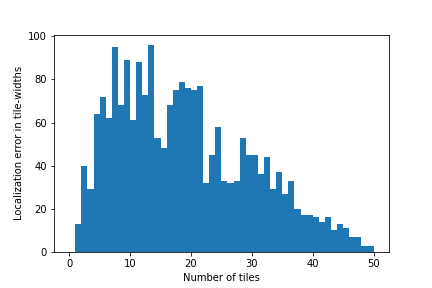
\includegraphics[width = 3.0in]{figures/thesis/plt_folder/rotate_hist_30}}&
		\subfloat[60 degrees error distribution]{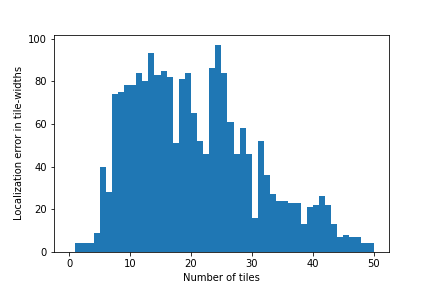
\includegraphics[width = 3.0in]{figures/thesis/plt_folder/rotate_hist_60}}\\
		\subfloat[90 degrees error distribution]{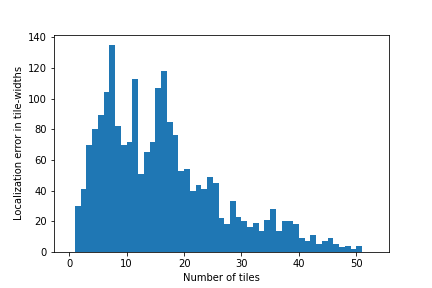
\includegraphics[width = 3.0in]{figures/thesis/plt_folder/rotate_hist_90}}&
		\subfloat[120 degrees error distribution]{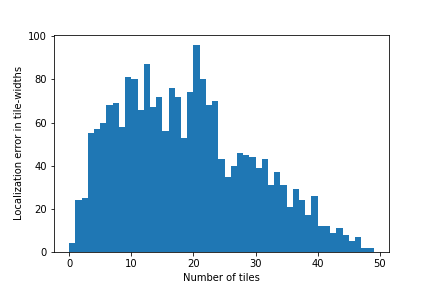
\includegraphics[width = 3.0in]{figures/thesis/plt_folder/rotate_hist_120}}\\
		\subfloat[150 degrees]{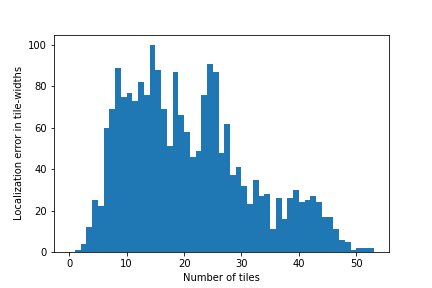
\includegraphics[width = 3.0in]{figures/thesis/plt_folder/rotate_hist_150}}&
		\subfloat[150 degrees error distribution]{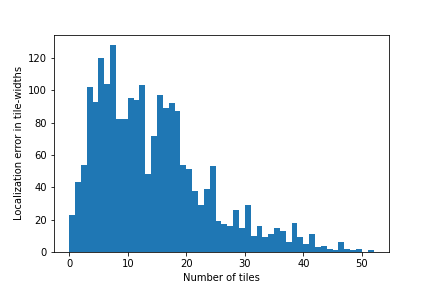
\includegraphics[width = 3.0in]{figures/thesis/plt_folder/rotate_hist_180}}\\
		\subfloat[180 degrees]{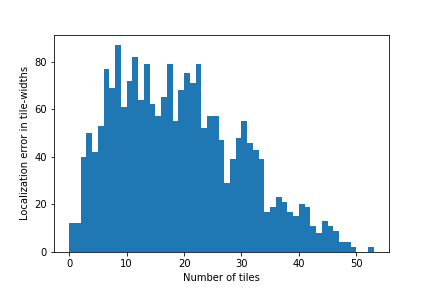
\includegraphics[width = 3.0in]{figures/thesis/plt_folder/rotate_hist_210}}&
		\subfloat[180 degrees error distribution]{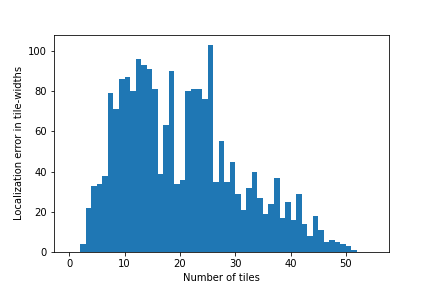
\includegraphics[width = 3.0in]{figures/thesis/plt_folder/rotate_hist_240}}\\
	\end{longtable}
\end{figure}


	\begin{figure}
	\begin{longtable}{cc}
		\subfloat[210 degrees]{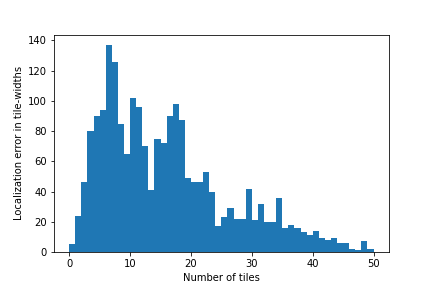
\includegraphics[width = 3.0in]{figures/thesis/plt_folder/rotate_hist_270}}&
		\subfloat[210 degrees error distribution]{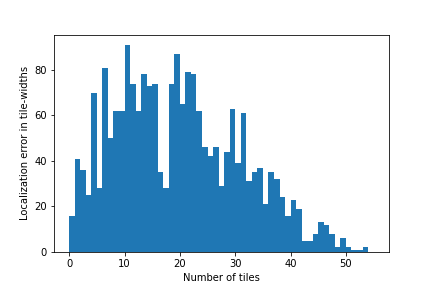
\includegraphics[width = 3.0in]{figures/thesis/plt_folder/rotate_hist_230}}\\
		\subfloat[270 degrees error distribution]{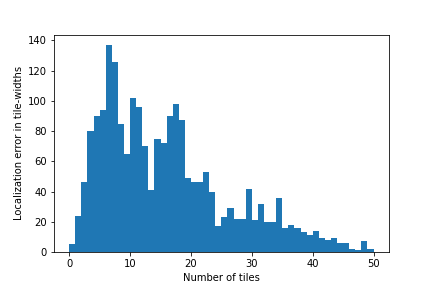
\includegraphics[width = 3.0in]{figures/thesis/plt_folder/rotate_hist_270}}&
		\subfloat[300 degrees]{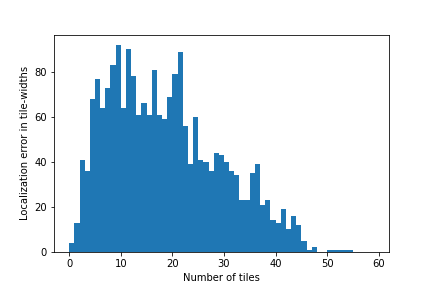
\includegraphics[width = 3.0in]{figures/thesis/plt_folder/rotate_hist_300}}\\
		\subfloat[300 degrees error distribution]{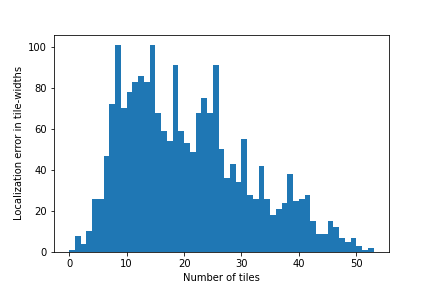
\includegraphics[width = 3.0in]{figures/thesis/plt_folder/rotate_hist_330}}
	\end{longtable}
	\caption{Effect of rotation on localization. We check the error for rotation steps of 30 degrees for the entire dataset, and show that as deviations from the actual orientation yields higher errors.}
	\label{Ev1.4}
\end{figure}

\newpage 
\subsubsection{Scaling}
Similarly, we vary the scale of the query tiles and check the prediction error statistics. The error plots below show clearly that the closer we get to the original scale, the lower the likelihood of an erroneous prediction (fig \ref{Ev1.5}). 

\begin{figure}
	\begin{longtable}{cc}
		\centering
		\subfloat[0.3 scaling error distribution]{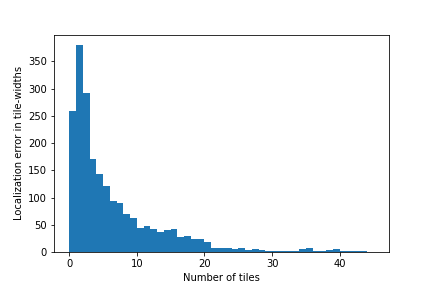
\includegraphics[width = 3.0in]{figures/thesis/plt_folder/scale_hist_0.3}}&
		\subfloat[0.7 scalings error distribution]{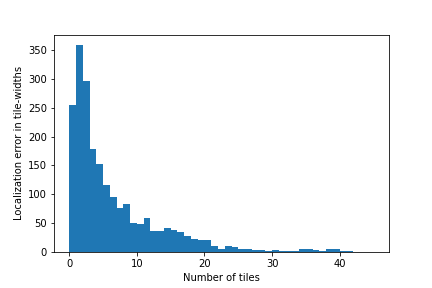
\includegraphics[width = 3.0in]{figures/thesis/plt_folder/scale_hist_0.7}}\\
		\subfloat[1.1 scaling error distribution]{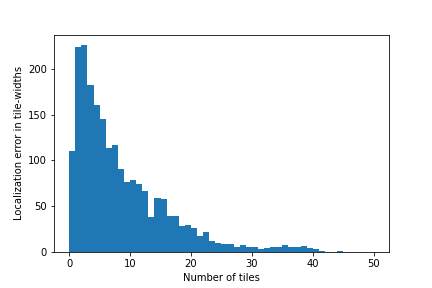
\includegraphics[width = 3.0in]{figures/thesis/plt_folder/scale_hist_1.1}}&
		\subfloat[1.5 scaling error distribution]{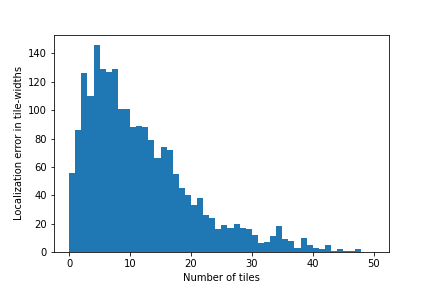
\includegraphics[width = 3.0in]{figures/thesis/plt_folder/scale_hist_1.5}}\\
		\subfloat[1.9 scaling error distribution]{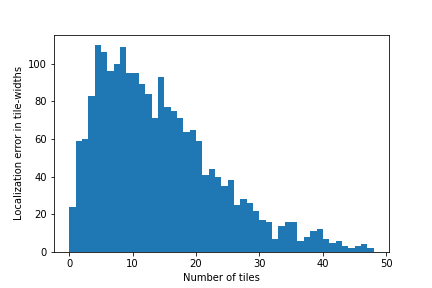
\includegraphics[width = 3.0in]{figures/thesis/plt_folder/scale_hist_1.9}}&
		\subfloat[2.3 scaling error distribution]{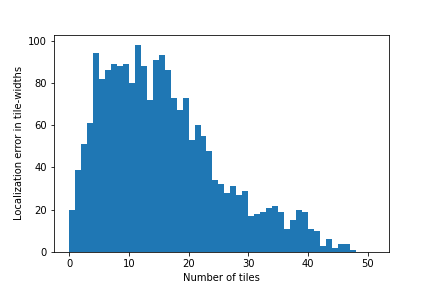
\includegraphics[width = 3.0in]{figures/thesis/plt_folder/scale_hist_2.3}}\\
		\subfloat[2.7 scaling error distribution]{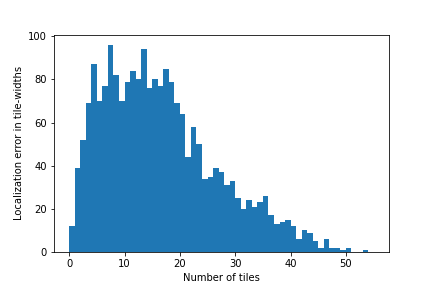
\includegraphics[width = 3.0in]{figures/thesis/plt_folder/scale_hist_2.7}}
	\end{longtable}
\end{figure}

\begin{figure}
	\caption{Effect of scaling on localization. We check the error for scaling steps of 0.4 scale increments for the entire dataset, and show that as deviations from the actual orientation yields higher errors.}
	\label{Ev1.5}
\end{figure}

\newpage
\subsection{Evaluation on query tiles constructed from the actual Oxford Sequence}

As we have stated, we evaluate our method on the Oxford Robotcar Dataset (\textcite{newman2017}). All the sequences of the RobotCar dataset are runs on a fixed route in different times and conditions. We choose the sequence \textbf{2015-03-17-11-08-44} for our evaluations (fig \ref{Ev1.7}).

\subsubsection{Evaluating for the Oxford RobotCar sequence}
For evaluation, we choose those locations in our oxford sequence that are as close as possible to those tiles in our training sequence that have a low localization error (within 1 tile distance). This way, we can make a fair evaluation in the sense that the locations we are testing from the Oxford Dataset are known to have done well when represented with standard OSM tiles.

Even though our Oxford Robotcar query locations will not overlap exactly with their corresponding OSM tiles of the training dataset, we can still make an evaluation of localization based on how close we can get to our OSM tile representation.

\myfig{thesis/oxford_dataset_traj.png}%% filename
{scale=0.25}%%oxford_dataset_traj.png width/height
{Trajectory of Oxford Dataset drive}%% caption
{Oxford dataset trajectory}%% optional (short) caption for list of figures
{Ev1.7}

We have sampled query locations almost uniformly from the oxford trajectory(fig \ref{Ev1.8}). We choose those locations with distinct building geometry, rejecting empty of nearly empty locations around a candidate query location.

We observe from the below figure that we have sampled locations uniformly from the original oxford driving trajectory. 

\myfig{thesis/query_dataset_traj.png}%% filename
{scale=0.3}%%oxford_dataset_traj.png width/height
{Query locations for evaluation}%% caption
{Query locations}%% optional (short) caption for list of figures
{Ev1.8}

As we have described in our methodology section, we create query map tiles at the locations shown above and evaluate how well the network localizes our query tiles at the locations sampled from the oxford robotcar trajectory ((fig \ref{Ev1.9})). We also separately show the localizations at different errors (fig \ref{Ev2.0}, fig \ref{Ev2.1}. fig \ref{Ev2.2}. fig \ref{Ev2.3}, fig \ref{Ev2.4}, fig \ref{Ev2.5})

We show below statistics of our system's performance:

\myfig{thesis/error_gps_query.png}%% filename
{scale=0.5}%%oxford_dataset_traj.png width/height
{Blue - GPS positions of ground truth. Red - GPS positions of prediction}%% caption
{Query prediction GPS}%% optional (short) caption for list of figures
{Ev1.9}

\myfig{thesis/pred_1.png}%% filename
{scale=0.3}%%oxford_dataset_traj.png width/height
{Blue - GPS positions of ground truth. Red - GPS positions of prediction. Locations with errors rounded to 1 Tile Width}%% caption
{Query prediction less than 1 Tile Width}%% optional (short) caption for list of figures
{Ev2.0}

\myfig{thesis/pred_2.png}%% filename
{scale=0.3}%%oxford_dataset_traj.png width/height
{Blue - GPS positions of ground truth. Red - GPS positions of prediction.Locations with errors rounded to 2 Tile Width}%% caption
{Query prediction less than 2 Tile Width}%% optional (short) caption for list of figures
{Ev2.1}

\myfig{thesis/pred_3.png}%% filename
{scale=0.3}%%oxford_dataset_traj.png width/height
{Blue - GPS positions of ground truth. Red - GPS positions of prediction. Locations with errors rounded to 3 Tile Width}%% caption
{Query prediction less than 3 Tile Width}%% optional (short) caption for list of figures
{Ev2.2}

\myfig{thesis/pred_4.png}%% filename
{scale=0.3}%%oxford_dataset_traj.png width/height
{Blue - GPS positions of ground truth. Red - GPS positions of prediction. Locations with errors rounded to 4 Tile Width}%% caption
{Query prediction less than 4 Tile Width}%% optional (short) caption for list of figures
{Ev2.3}

\myfig{thesis/pred_5.png}%% filename
{scale=0.3}%%oxford_dataset_traj.png width/height
{Blue - GPS positions of ground truth. Red - GPS positions of prediction. Locations with errors rounded to 5 Tile Width}%% caption
{Query prediction less than 5 Tile Width}%% optional (short) caption for list of figures
{Ev2.4}

\myfig{thesis/pred_6.png}%% filename
{scale=0.3}%%oxford_dataset_traj.png width/height
{Blue - GPS positions of ground truth. Red - GPS positions of prediction. Locations with errors rounded to 6 Tile Width}%% caption
{Query prediction less than 6 Tile Width}%% optional (short) caption for list of figures
{Ev2.5}

\myfig{thesis/error_hist_query.png}%% filename
{scale=1.0}%%oxford_dataset_traj.png width/height
{Localization error distribution over 237 locations in Oxford Trajectory}%% caption
{Query prediction error distribution}%% optional (short) caption for list of figures
{Ev2.6}

We observe that the predictions are within 6 tile widths of the ground truth (fig \ref{Ev2.6}). However, it has to be noted that we are able to narrow down the location to within a 6 tile radius (a search space of at most 91 tiles), given that the total search space is approximately 2500 tiles. 

\newpage
\subsubsection{A qualitative evaluation of the results}
We display here a set of (constructed tile, predicted tile) pairs to get a sense of how exactly the MapNet pose regressor behaves in this setting. (fig \ref{Ev2.7}, fig \ref{Ev2.8}, fig \ref{Ev2.9}, fig \ref{Ev3.0}, fig \ref{Ev3.1}, fig \ref{Ev3.2})

\begin{figure}
	\centering
    \figuretitle{Examples with Localization errors less than 1 Tile Width}
	\begin{longtable}{cc}
		\subfloat{
\includegraphics[width = 1.5in]{figures/thesis/evals/1.0/1_gt.png}}&
		\subfloat{
\includegraphics[width = 1.5in]{figures/thesis/evals/1.0/1_pred.png}}\\
		\subfloat{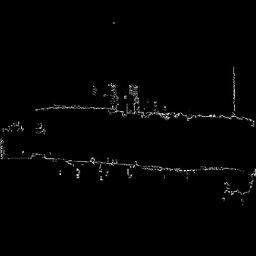
\includegraphics[width = 1.5in]{figures/thesis/evals/1.0/2_gt.png}} &
		\subfloat{
\includegraphics[width = 1.5in]{figures/thesis/evals/1.0/2_pred.png}}\\
		\subfloat{
\includegraphics[width = 1.5in]{figures/thesis/evals/1.0/3_gt.png}} &
		\subfloat{
\includegraphics[width = 1.5in]{figures/thesis/evals/1.0/3_pred.png}}\\
		\subfloat{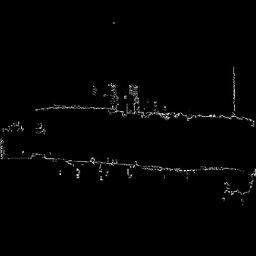
\includegraphics[width = 1.5in]{figures/thesis/evals/1.0/4_gt.png}}&
		\subfloat{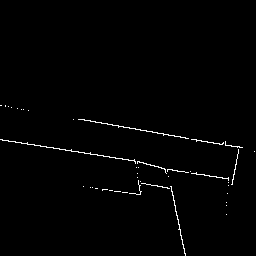
\includegraphics[width = 1.5in]{figures/thesis/evals/1.0/4_pred.png}}\\
	\end{longtable}
\end{figure}

\begin{figure}
	\begin{longtable}{cc}
		\subfloat{
\includegraphics[width = 1.5in]{figures/thesis/evals/1.0/5_gt.png}}&
		\subfloat{
\includegraphics[width = 1.5in]{figures/thesis/evals/1.0/5_pred.png}}
	\end{longtable}
	\caption{Left - query tile, Right - Predicted tile on raster. We note that the prediction manages to find structure quite similar to the kind of structure present in the query tiles. Note that as long as noise conforms somewhat to the true contours of the buildings around them, we get a good prediction that is close to the location of the query tile. Note that the scaling of the query tile and OSM tile doesn't exactly match up. This is mainly because we get our scale factor by scaling the metric distance travelled on road to the metric resolution of the typical OSM tile.}
	\label{Ev2.7}
\end{figure}

\begin{figure}
	\centering
	\figuretitle{Examples with Localization errors between 1 and 2 Tile Widths}
	\begin{longtable}{cc}
	    \subfloat{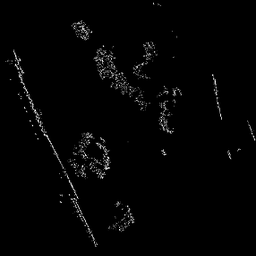
\includegraphics[width = 1.5in]{figures/thesis/evals/2.0/1_gt.png}}&
		\subfloat{
\includegraphics[width = 1.5in]{figures/thesis/evals/2.0/1_pred.png}}\\
		\subfloat{
\includegraphics[width = 1.5in]{figures/thesis/evals/2.0/2_gt.png}} &
		\subfloat{
\includegraphics[width = 1.5in]{figures/thesis/evals/2.0/2_pred.png}}\\
		\subfloat{
\includegraphics[width = 1.5in]{figures/thesis/evals/2.0/3_gt.png}} &
		\subfloat{
\includegraphics[width = 1.5in]{figures/thesis/evals/2.0/3_pred.png}}\\
	    \subfloat{
\includegraphics[width = 1.5in]{figures/thesis/evals/2.0/4_gt.png}}&
		\subfloat{
\includegraphics[width = 1.5in]{figures/thesis/evals/2.0/4_pred.png}}\\
	\end{longtable}
\end{figure}

\begin{figure}
	\begin{longtable}{cc}
		\subfloat{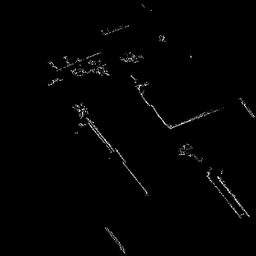
\includegraphics[width = 1.5in]{figures/thesis/evals/2.0/5_gt.png}}&
		\subfloat{
\includegraphics[width = 1.5in]{figures/thesis/evals/2.0/5_pred.png}}
	\end{longtable}
	\caption{Left - query tile, Right - Predicted tile on raster. Looking at a few tiles with localization error of less than 2 tile widths, we observe that the network predicts tiles with similar structures which conform well to the original structure but are led astray by noise. }
	\label{Ev2.8}
\end{figure}

\begin{figure}
    \centering
    \figuretitle{Examples with Localization errors between 2 and 3 Tile Widths}
	\begin{longtable}{cc}
		\subfloat{
\includegraphics[width = 1.5in]{figures/thesis/evals/3.0/1_gt.png}}&
		\subfloat{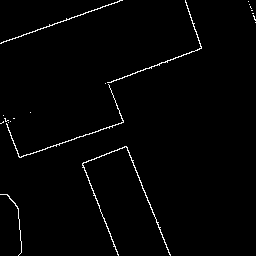
\includegraphics[width = 1.5in]{figures/thesis/evals/3.0/1_pred.png}}\\
		\subfloat{
\includegraphics[width = 1.5in]{figures/thesis/evals/3.0/2_gt.png}} &
		\subfloat{
\includegraphics[width = 1.5in]{figures/thesis/evals/3.0/2_pred.png}}\\
		\subfloat{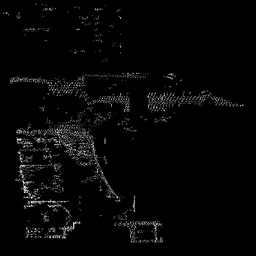
\includegraphics[width = 1.5in]{figures/thesis/evals/3.0/3_gt.png}} &
		\subfloat{
\includegraphics[width = 1.5in]{figures/thesis/evals/3.0/3_pred.png}}\\
		\subfloat{
\includegraphics[width = 1.5in]{figures/thesis/evals/3.0/4_gt.png}}&
		\subfloat{
\includegraphics[width = 1.5in]{figures/thesis/evals/3.0/4_pred.png}}
	\end{longtable}
\end{figure}

\begin{figure}
	\begin{longtable}{cc}
		\subfloat{\includegraphics[width = 1.5in]{figures/thesis/evals/3.0/5_gt.png}}&
		\subfloat{\includegraphics[width = 1.5in]{figures/thesis/evals/3.0/5_pred.png}}
	\end{longtable}
	\caption{Left - query tile, Right - Predicted tile on raster. We still observe that the predictions are structurally similar to query tiles, but cannot be on point thanks to the noise contributed by trees segmented as buildings. Note that the scaling of the query tile and OSM tile doesn't exactly match up. This is mainly because we get our scale factor by scaling the metric distance travelled on road to the metric resolution of the typical OSM tile}
	\label{Ev2.9}
\end{figure}

\begin{figure}
	\centering
	\figuretitle{Examples with Localization errors between 3 and 4 Tile Widths}
	\begin{longtable}{cc}
		\subfloat{\includegraphics[width = 1.5in]{figures/thesis/evals/4.0/1_gt.png}}&
		\subfloat{\includegraphics[width = 1.5in]{figures/thesis/evals/4.0/1_pred.png}}\\
		\subfloat{\includegraphics[width = 1.5in]{figures/thesis/evals/4.0/2_gt.png}} &
		\subfloat{\includegraphics[width = 1.5in]{figures/thesis/evals/4.0/2_pred.png}}\\
		\subfloat{\includegraphics[width = 1.5in]{figures/thesis/evals/4.0/3_gt.png}} &
		\subfloat{\includegraphics[width = 1.5in]{figures/thesis/evals/4.0/3_pred.png}}\\
		\subfloat{\includegraphics[width = 1.5in]{figures/thesis/evals/4.0/4_gt.png}}&
		\subfloat{\includegraphics[width = 1.5in]{figures/thesis/evals/4.0/4_pred.png}}
	\end{longtable}
\end{figure}

\begin{figure}
	\begin{longtable}{cc}
		\subfloat{\includegraphics[width = 1.5in]{figures/thesis/evals/4.0/5_gt.png}}&
		\subfloat{\includegraphics[width = 1.5in]{figures/thesis/evals/4.0/5_pred.png}}
	\end{longtable}
	\caption{Left - query tile, Right - Predicted tile on raster. Structural similarity is still observable in the predictions, but noise confuses the network because it doesn't conform to the true building outline to give a good enough prediction.Note that the scaling of the query tile and OSM tile doesn't exactly match up. This is mainly because we get our scale factor by scaling the metric distance travelled on road to the metric resolution of the typical OSM tile}
	\label{Ev3.0}
\end{figure}

\begin{figure}
	\centering
    \figuretitle{Examples with Localization errors between 4 and 5 Tile Widths}
	\begin{longtable}{cc}
		\subfloat{\includegraphics[width = 1.5in]{figures/thesis/evals/5.0/1_gt.png}}&
		\subfloat{\includegraphics[width = 1.5in]{figures/thesis/evals/5.0/1_pred.png}}\\
		\subfloat{\includegraphics[width = 1.5in]{figures/thesis/evals/5.0/2_gt.png}} &
		\subfloat{\includegraphics[width = 1.5in]{figures/thesis/evals/5.0/2_pred.png}}\\
		\subfloat{\includegraphics[width = 1.5in]{figures/thesis/evals/5.0/3_gt.png}} &
		\subfloat{\includegraphics[width = 1.5in]{figures/thesis/evals/5.0/3_pred.png}}\\
		\subfloat{\includegraphics[width = 1.5in]{figures/thesis/evals/5.0/4_gt.png}}&
		\subfloat{\includegraphics[width = 1.5in]{figures/thesis/evals/5.0/4_pred.png}}
	\end{longtable}
\end{figure}

\begin{figure}
	\begin{longtable}{cc}
		\subfloat{\includegraphics[width = 1.5in]{figures/thesis/evals/5.0/5_gt.png}}&
		\subfloat{\includegraphics[width = 1.5in]{figures/thesis/evals/5.0/5_pred.png}}
	\end{longtable}
	\caption{Left - query tile, Right - Predicted tile on raster. Structural similarity is still observable in the predictions, but noise confuses the network because it doesn't conform to the true building outline to give a good enough prediction. Note that the scaling of the query tile and OSM tile doesn't exactly match up. This is mainly because we get our scale factor by scaling the metric distance travelled on road to the metric resolution of the typical OSM tile}
	\label{Ev3.1}
\end{figure}
 

\begin{figure}
	\centering
    \figuretitle{Examples with Localization errors between 5 and 6 Tile Widths}
	\begin{longtable}{cc}
		\subfloat{\includegraphics[width = 1.5in]{figures/thesis/evals/6.0/1_gt.png}}&
		\subfloat{\includegraphics[width = 1.5in]{figures/thesis/evals/6.0/1_pred.png}}\\
		\subfloat{\includegraphics[width = 1.5in]{figures/thesis/evals/6.0/2_gt.png}} &
		\subfloat{\includegraphics[width = 1.5in]{figures/thesis/evals/6.0/2_pred.png}}\\
		\subfloat{\includegraphics[width = 1.5in]{figures/thesis/evals/6.0/3_gt.png}} &
		\subfloat{\includegraphics[width = 1.5in]{figures/thesis/evals/6.0/3_pred.png}}\\
		\subfloat{\includegraphics[width = 1.5in]{figures/thesis/evals/6.0/4_gt.png}}&
		\subfloat{\includegraphics[width = 1.5in]{figures/thesis/evals/6.0/4_pred.png}}
	\end{longtable}
\end{figure}

\begin{figure}
	\begin{longtable}{cc}
		\subfloat{\includegraphics[width = 1.5in]{figures/thesis/evals/6.0/5_gt.png}}&
		\subfloat{\includegraphics[width = 1.5in]{figures/thesis/evals/6.0/5_pred.png}}
	\end{longtable}
	\caption{Left - query tile, Right - Predicted tile on raster. Structural similarity is still observable in the predictions, but noise confuses the network because it doesn't conform to the true building outline to give a good enough prediction. Note that the scaling of the query tile and OSM tile doesn't exactly match up. This is mainly because we get our scale factor by scaling the metric distance travelled on road to the metric resolution of the typical OSM tile}
	\label{Ev3.2}
\end{figure}





  
\chapter{Conclusion}
We have demonstrated in our work thus far that we can localize directly a car driving through an urban locale directly upon a map raster of that area. We have shown that a pose regression network trained with overlapping tiles of some map area is able to localize the car's position, given a query map tile constructed from the scene. We've shown also a method to create a suitable training OSM tile set for a given area, taking into account issues such as the car's vield of view.

This being an initial formulation of the approach, we outlined how to construct the query map tile using labeled pointclouds. We've also described an approach to mitigating noise in the labeling of the pointcloud, which leads to an improved query map tile construction. 

\subsection{Future Work}
The route we take to make the our query tiles exactly similar in content, scale and orientation to the Open Street Map tile at that location is not necessarily always robust. This is due to inaccuracies in transferring image labels to the pointcloud, and as mapping pixel/metre resolution of query tile to road resolution is not always accurate as we have access only to the distance travelled on the road.
	
As we have proved before in our evaluation section, such perturbations will lead to a noisy predictions. 

In the future, we aim to improve the pipeline to function at a production level in the following possible ways:

\begin{itemize}
\item We can make the pose regression network robust to possibly noisy tiles. A possible way to deal with this problem is to train a Convolutional Neural Network to filter out the noisy top-down projection of the pointcloud to produce a clean query map tile, or train our Pose Regression network to be robust to noisy tiles during pose inference.
\\
\item To deal with inaccurate scaling, it is desirable to either incorporate data augmentation with scaling during training or rework the backbone network to be more robust to the scale variations of map tiles. 
\\
\item Instead of focusing on being robust to noise, we can take the route of utilizing the now-popular pointcloud segmentation networks to directly get less noisier labelings of our LIDAR pointclouds. This will implicitly lead to more accurate query map-tile creations.
\\
\item Finally, we can do a more exhaustive hyperparameter search on the existing network parameters and tune the existing architecture of MapNet to better suit the specific problem of regressing pose off OSM tiles. The overlap between tiles while creating the training dataset will definitely have a strong influence on the results, and its effect must be explored more exhaustively. 
\end{itemize}

            
%%%%%% Time-stamp: <2012-08-20 17:41:39 vk>

%% example text content
%% scrartcl and scrreprt starts with section, subsection, subsubsection, ...
%% scrbook starts with part (optional), chapter, section, ...
%%\chapter{Example Chapter}

\chapter{Introduction}

This is my text with an example Figure~\ref{fig:example} and example
citation~\cite{StrunkWhite} or \textcite{Bringhurst1993}. And there is another
\enquote{citation} which is located at the bottom\footcite{tagstore}.

\myfig{TU_Graz_Logo}%% filename in figures folder
  {width=0.1\textwidth,height=0.1\textheight}%% maximum width/height, aspect ratio will be kept
  {Example figure.}%% caption
  {}%% optional (short) caption for table of figures
  {fig:example}%% label

Now you are able to write your own document. Always keep in mind: it's
the \emph{content} that matters, not the form. But good typography is
able to deliver the content much better than information set with bad
typography. This template allows you to focus on writing good content
while the form is done by the template definitions.


%% vim:foldmethod=expr
%% vim:fde=getline(v\:lnum)=~'^%%%%\ .\\+'?'>1'\:'='
%%% Local Variables: 
%%% mode: latex
%%% mode: auto-fill
%%% mode: flyspell
%%% eval: (ispell-change-dictionary "en_US")
%%% TeX-master: "main"
%%% End: 
 
%%\input{example-style-chapter}   %% remove this line to get rid of the style chapter

%% include tex file chapters:
% \include{introduction}        %% this is a suggestion: you have to create this file on demand
% \include{problem}             %% this is a suggestion: you have to create this file on demand
% \include{solution}            %% this is a suggestion: you have to create this file on demand
% \include{evaluation}          %% this is a suggestion: you have to create this file on demand
% \include{outlook}             %% this is a suggestion: you have to create this file on demand

\appendix                       %% closes main document, appendix follows until end; only available in book-classes
\addpart*{Appendix}             %% adding Appendix to tableofcontents

\printbibliography              %% remove, if using BibTeX instead of biblatex
% \include{further_ressources}  %% this is a suggestion: you have to create this file on demand

%%%% end{document}
\end{document}
%% vim:foldmethod=expr
%% vim:fde=getline(v\:lnum)=~'^%%%%\ .\\+'?'>1'\:'='
%%% Local Variables:
%%% mode: latex
%%% mode: auto-fill
%%% mode: flyspell
%%% eval: (ispell-change-dictionary "en_US")
%%% TeX-master: "main"
%%% End:
